\section{Simulation}
\subsection{First Study}

For the first simulation exercise, we simulate a dataset with 150 observations.

We set the true parameter values as $ \beta = 2 $, $ \gamma = 0 $, $ \delta = -1 $, $ \pi = 2 $, and $ \phi = 1 $. In our case, $W$ is a vector of ones. The covariance matrix of the errors is specified as
\begin{align*}
\Sigma = \begin{pmatrix}
1 & 0.5 \\
0.5 & 1
\end{pmatrix}.
\end{align*}

Our priors are set as follows: 
\begin{itemize}
    \item $\bftau \sim \mathcal{N}((0,0)', \mathrm{diag}(10,10))$,
    \item $\bftheta \sim \mathcal{N}((0,0,0)', \mathrm{diag}(10, 0.0001, 10))$,
    \item $\Sigma \sim \mathcal{IW}(3, I_2)$.
\end{itemize}

We run the Gibbs sampler for 10,000 iterations, discarding the first 5,000 as burn-in. The results are summarized in Table \ref{tab:simulation_results}.


% Table created by stargazer v.5.2.3 by Marek Hlavac, Social Policy Institute. E-mail: marek.hlavac at gmail.com
% Date and time: Mon, Apr 28, 2025 - 11:47:58 PM
\begin{table}[!htbp] \centering 
  \caption{Simulation Results} 
  \label{tab:simulation_results} 
\begin{tabular}{@{\extracolsep{5pt}} ccccccc} 
\\[-1.8ex]\hline 
\hline \\[-1.8ex] 
Parameter & True Value & Mean & Standard Deviation & 0.025 & 0.975 & Effective Sample Size \\ 
\hline \\[-1.8ex] 
pi & $2$ & $1.86$ & $0.09$ & $1.69$ & $2.03$ & $7,509.79$ \\ 
phi & $1$ & $1.03$ & $0.08$ & $0.87$ & $1.18$ & $7,723.48$ \\ 
beta & $2$ & $1.89$ & $0.10$ & $1.70$ & $2.09$ & $10,813.67$ \\ 
gamma & $0$ & $0.00$ & $0.01$ & $$-$0.02$ & $0.02$ & $6,469.12$ \\ 
delta & $$-$1$ & $$-$0.84$ & $0.21$ & $$-$1.27$ & $$-$0.44$ & $8,566.37$ \\ 
\hline \\[-1.8ex] 
\end{tabular} 
\end{table} 


The traceplot in Figure \ref{fig:simulation_traceplot} shows the evolution of the Markov chain for the parameters. No evident trends or drifts are present, suggesting that the Gibbs sampler has converged to the stationary posterior distribution.

\begin{figure}[H]
\centering
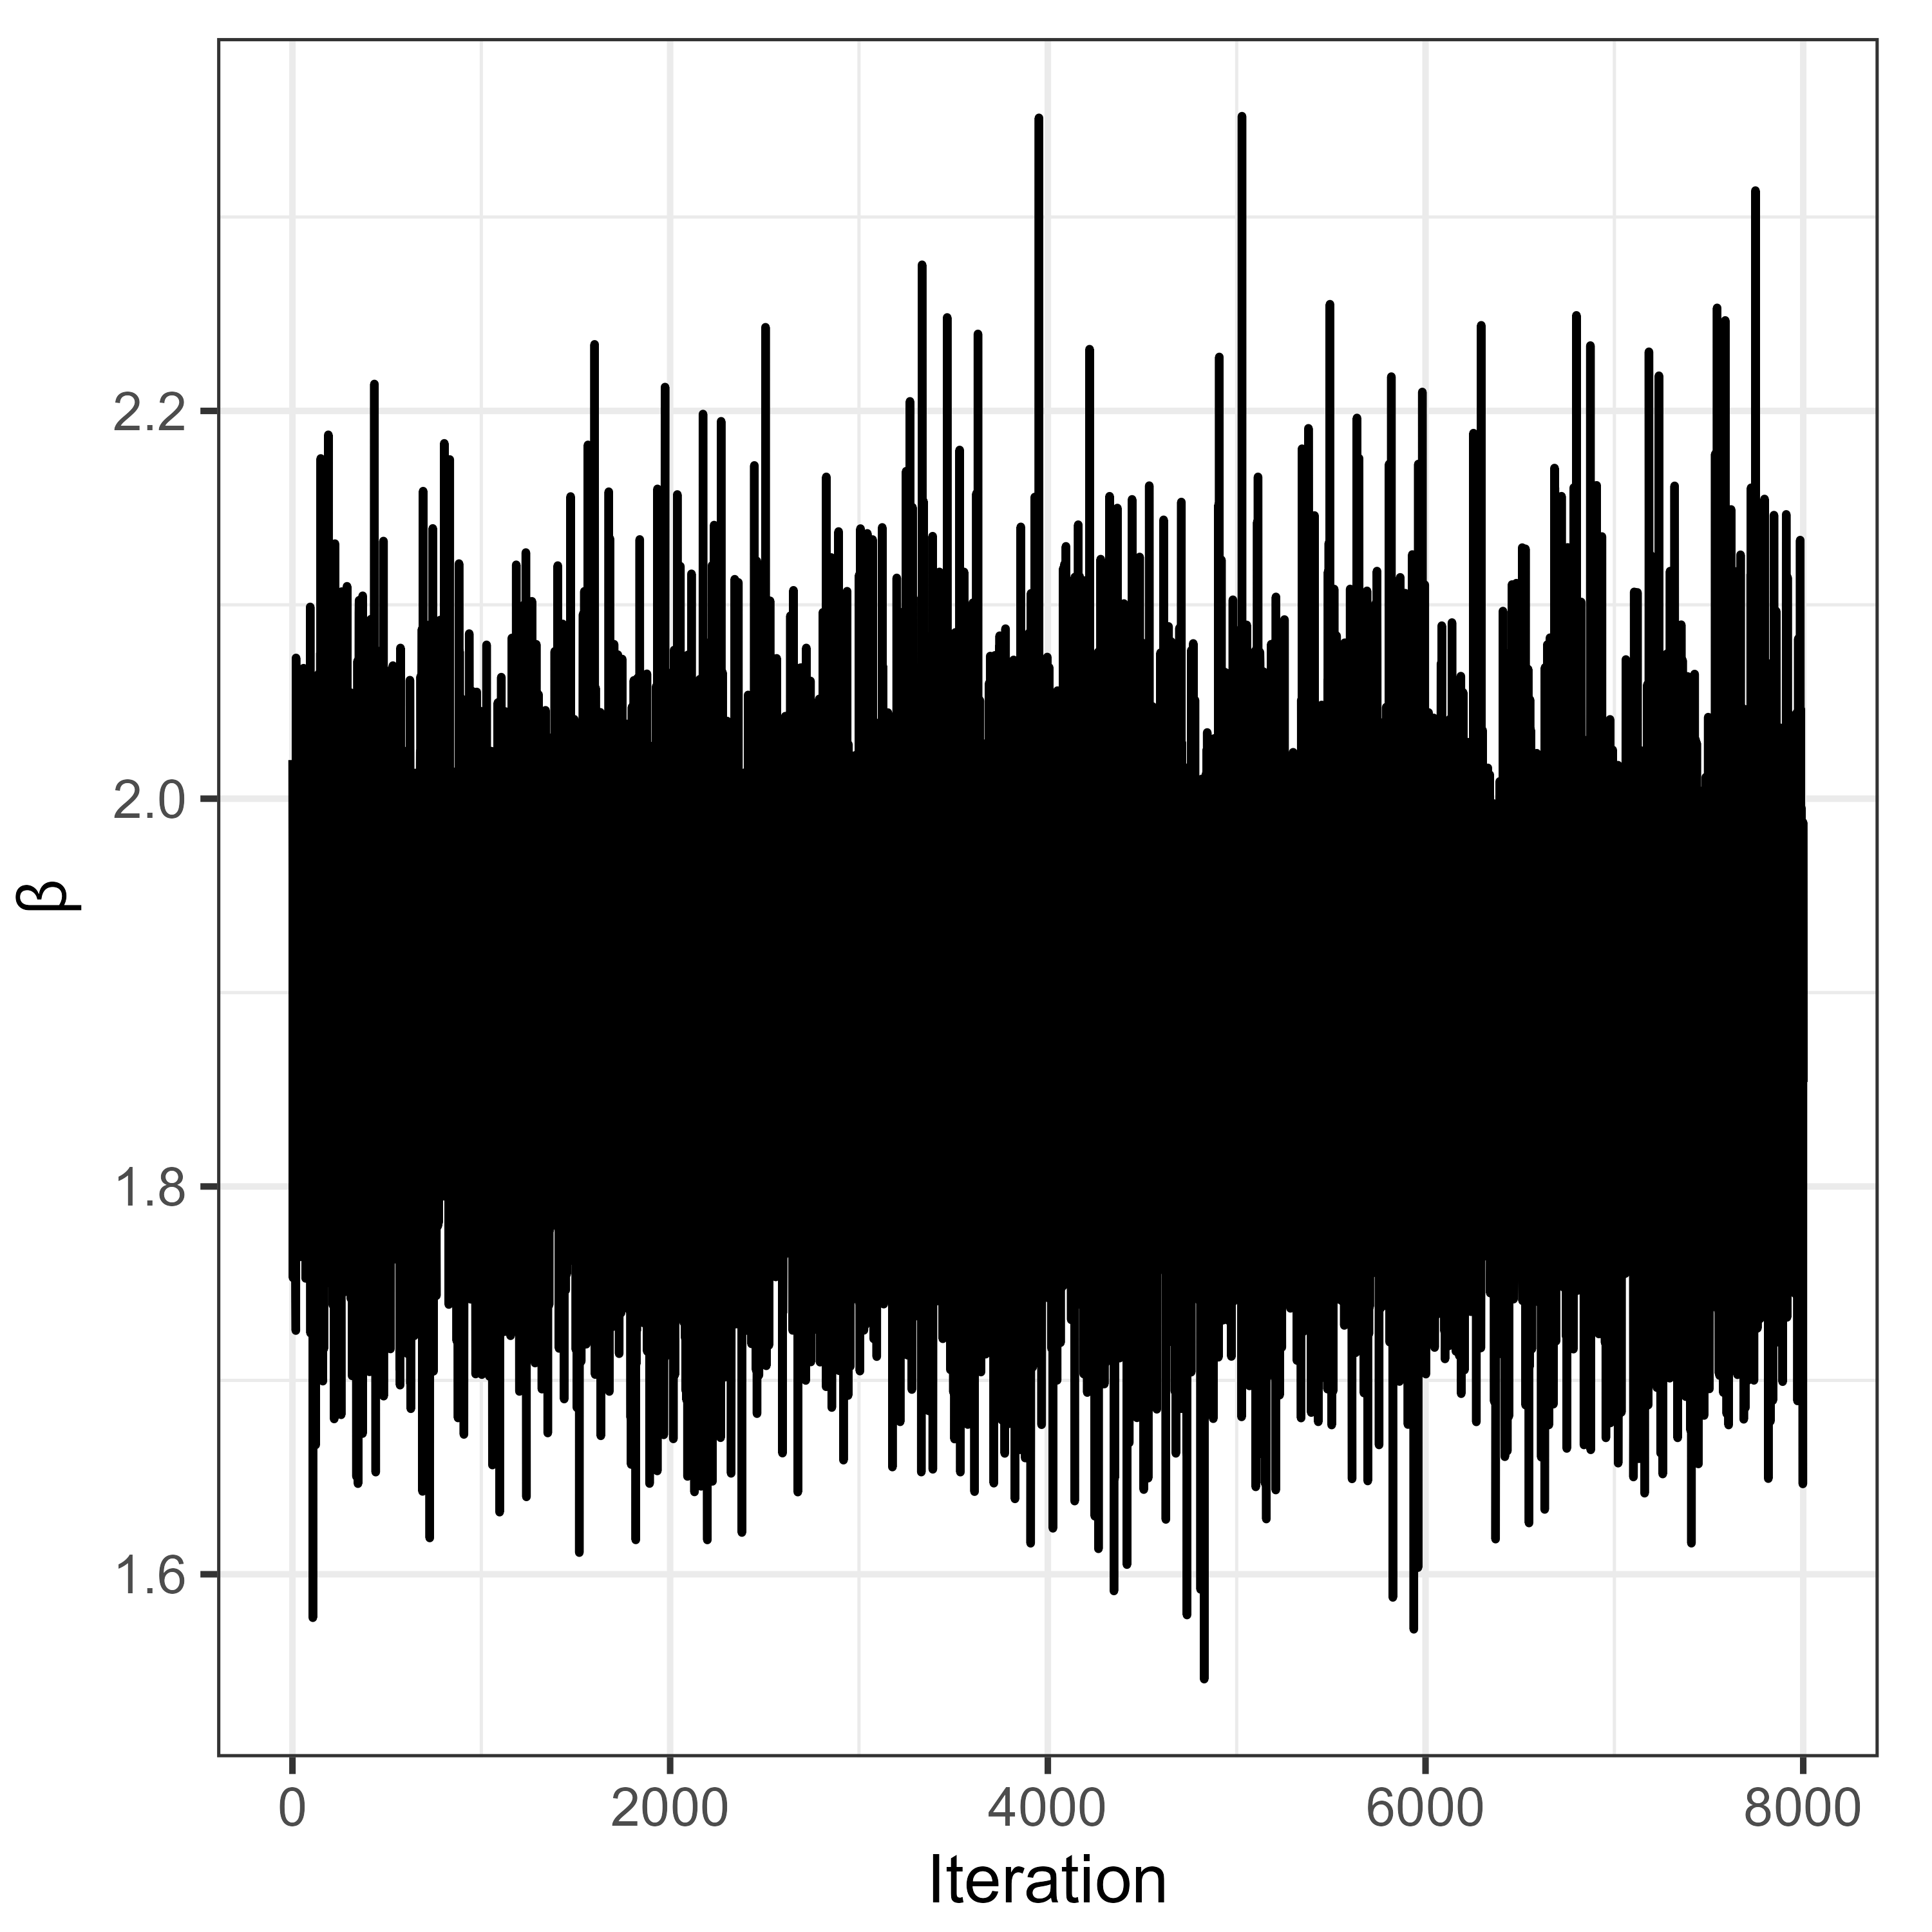
\includegraphics[width=0.6\textwidth]{../figures/simulation/trace_beta.png}
\caption{Traceplot of $\beta$ --- Simulation Study}
\label{fig:simulation_traceplot}
\end{figure}

The autocorrelation plot in Figure \ref{fig:simulation_autocorrelation} demonstrates low autocorrelation across lags, indicating good mixing of the Markov chain.

\begin{figure}[H]
\centering
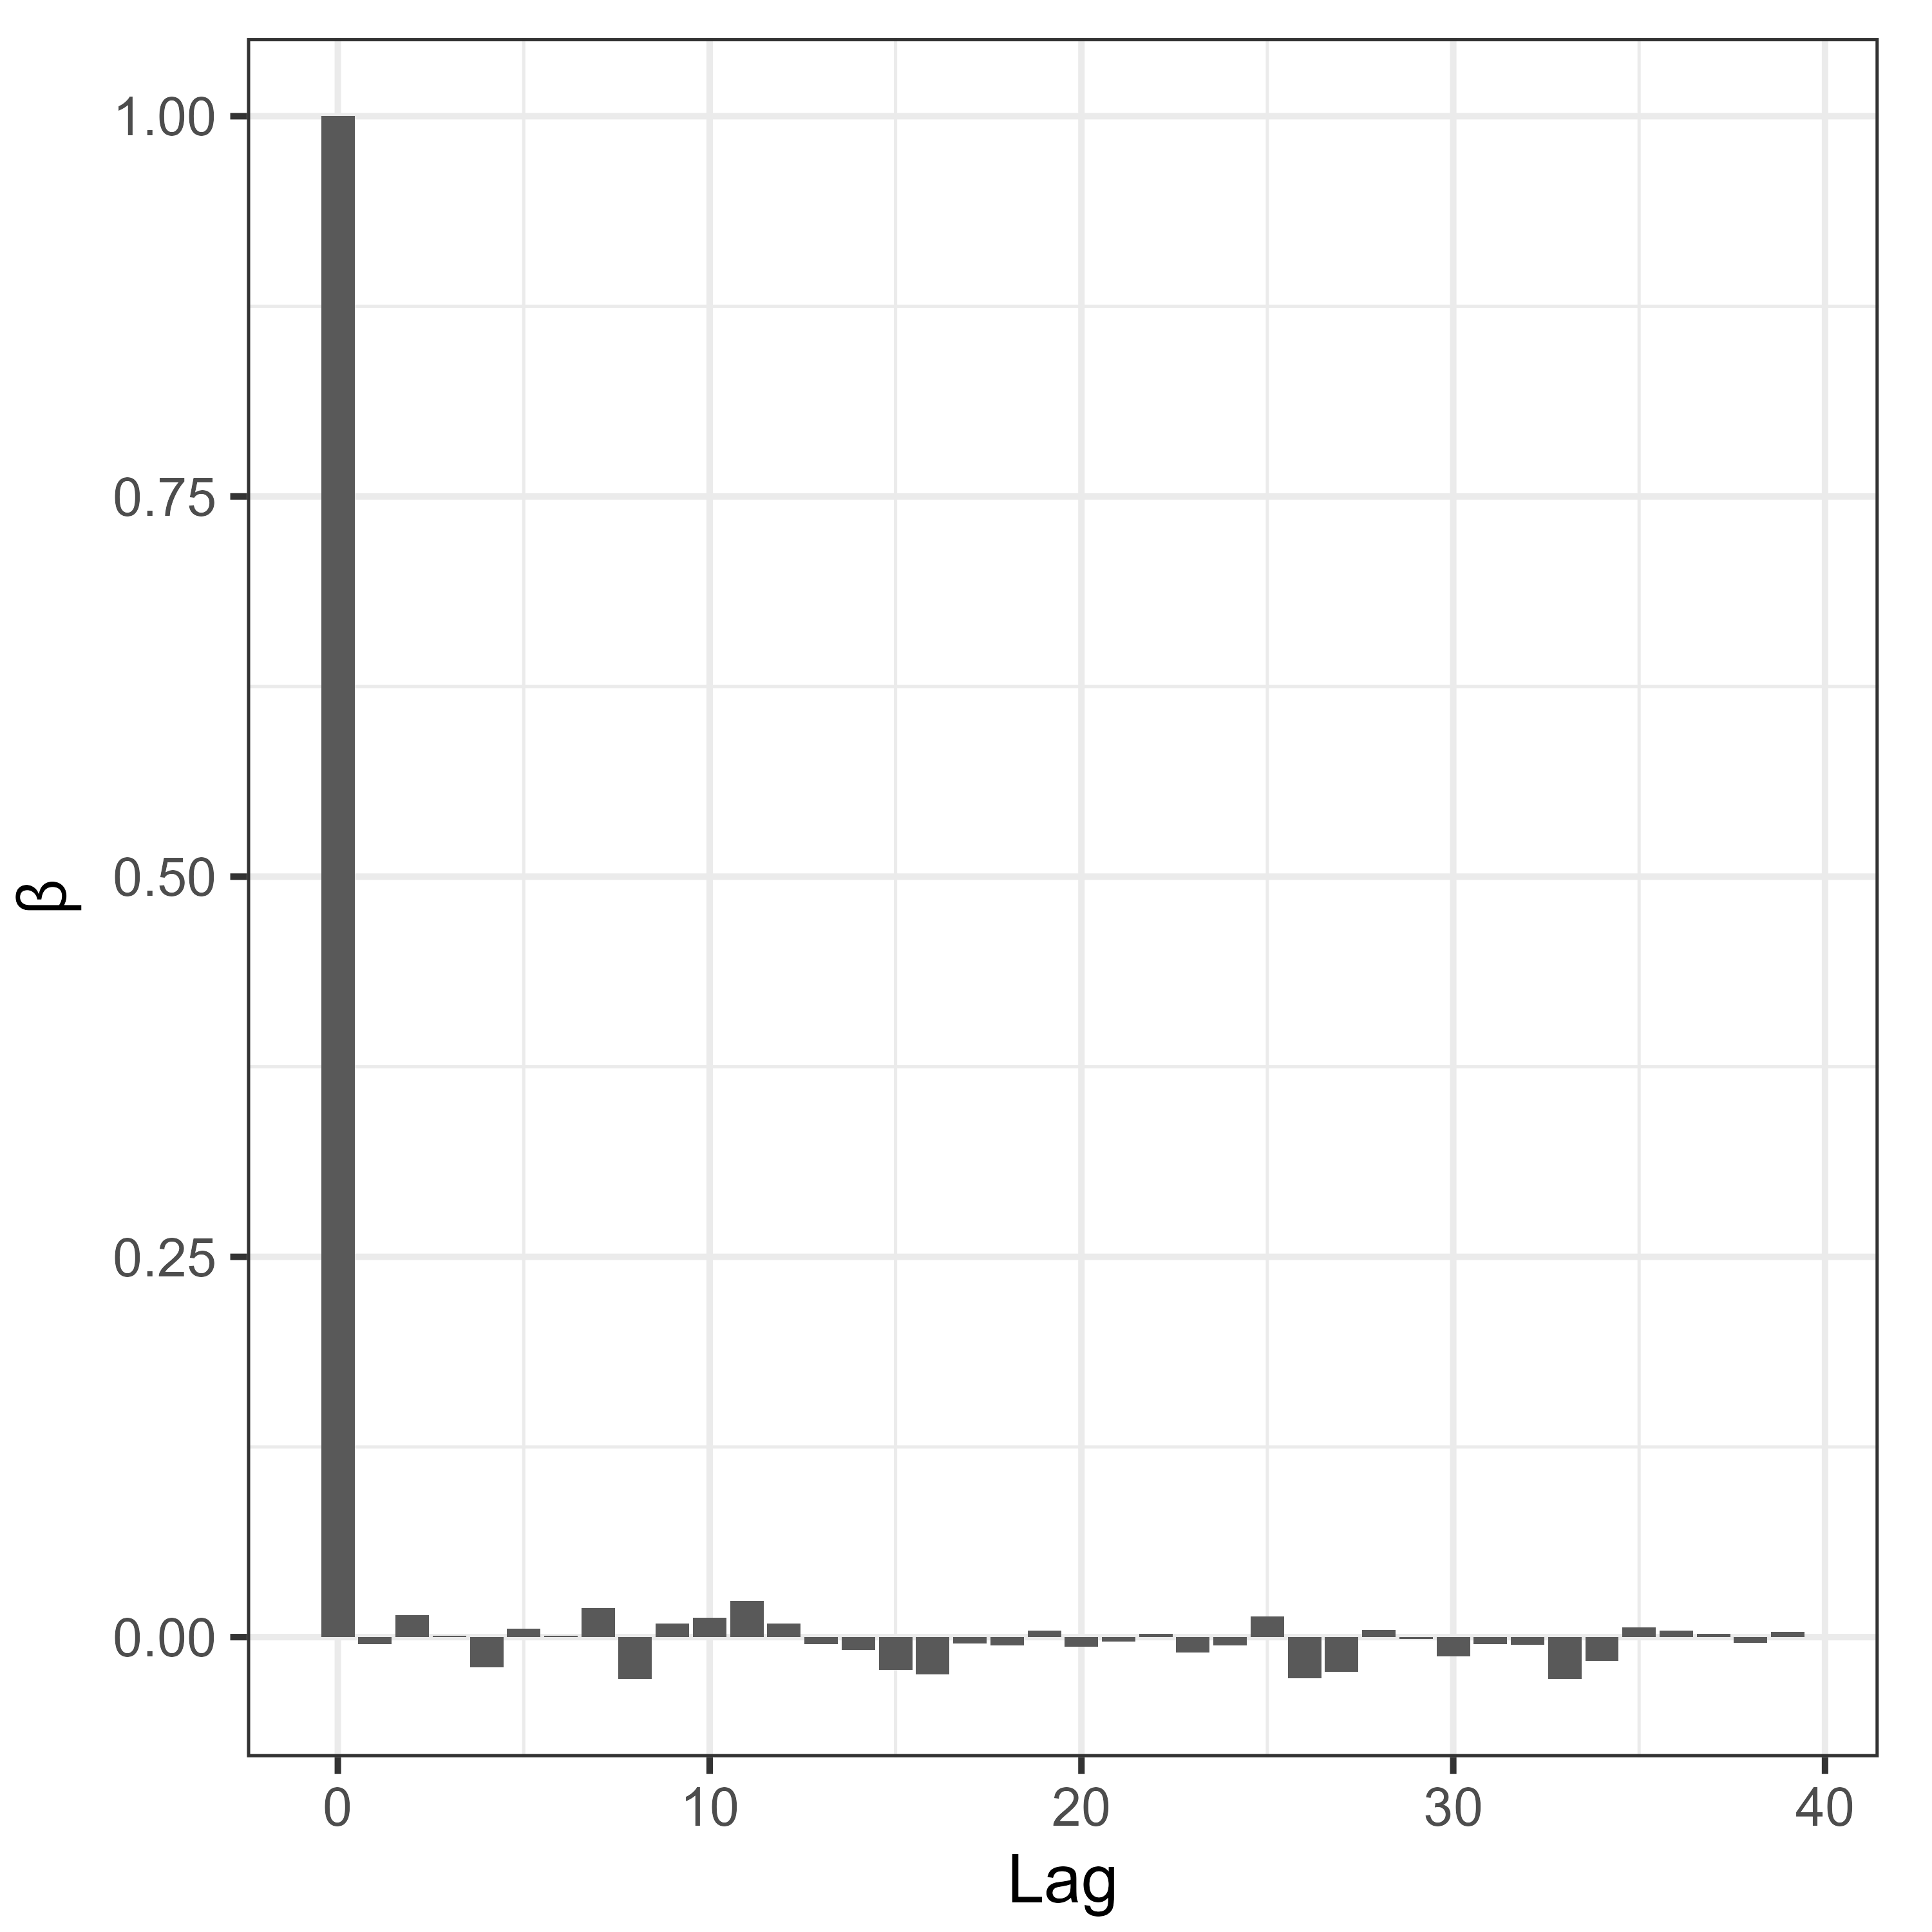
\includegraphics[width=0.6\textwidth]{../figures/simulation/acf_beta.png}
\caption{Autocorrelation of $\beta$ --- Simulation Study}
\label{fig:simulation_autocorrelation}
\end{figure}

We also plot the posterior distributions of the parameters in Figure \ref{fig:posterior_distributions} through histograms.

\begin{figure}[H]
\centering
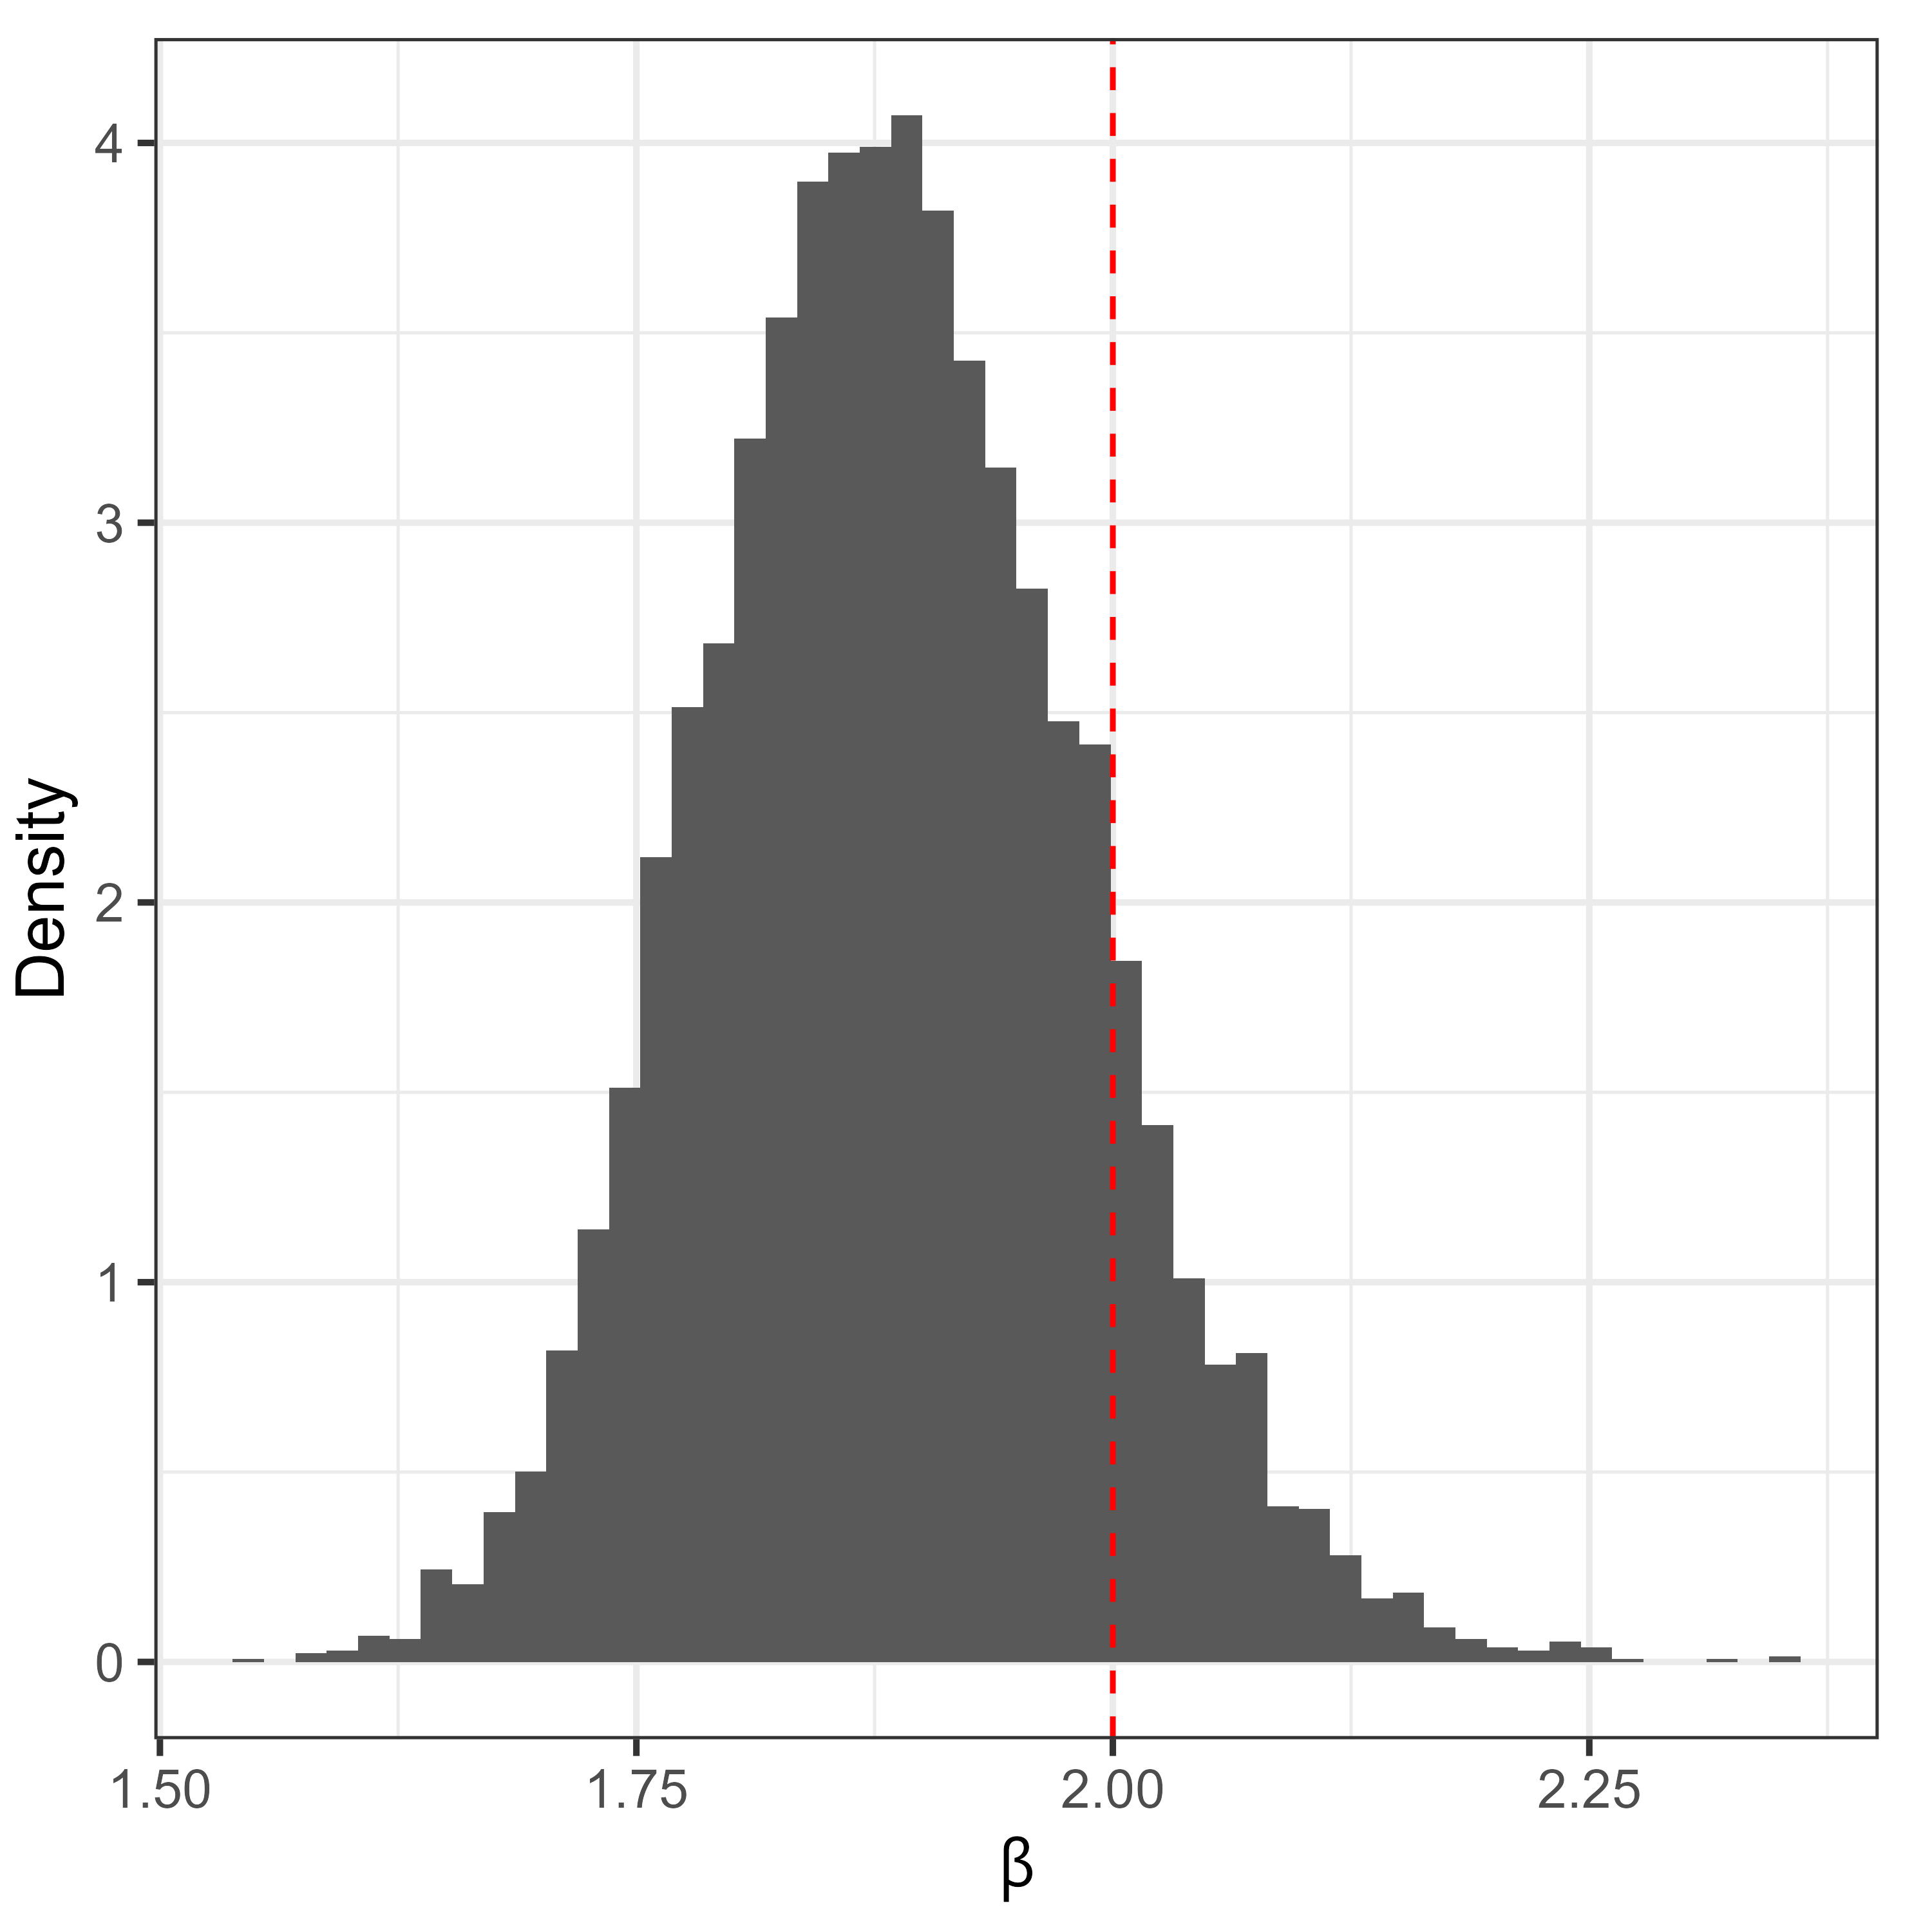
\includegraphics[width=0.6\textwidth]{../figures/simulation/hist_beta.png}
\caption{Posterior Distribution of $\beta$ --- Simulation Study}
\label{fig:posterior_distributions}
\end{figure}

As shown, the posterior distributions are centered close to the true parameter values, with minor deviations. This indicates that the Gibbs sampler successfully recovers the true parameters of the model under the simulated setting. As our sample size is relatively small, we would not expect to see a perfect recovery of the true parameters, but we cannot differentiate between the true and the estimated parameters. 

The other parameters also have a satisfactory recovery, as shown in Table \ref{tab:simulation_results} and the following figures. 

\begin{figure}[H]
    \centering
    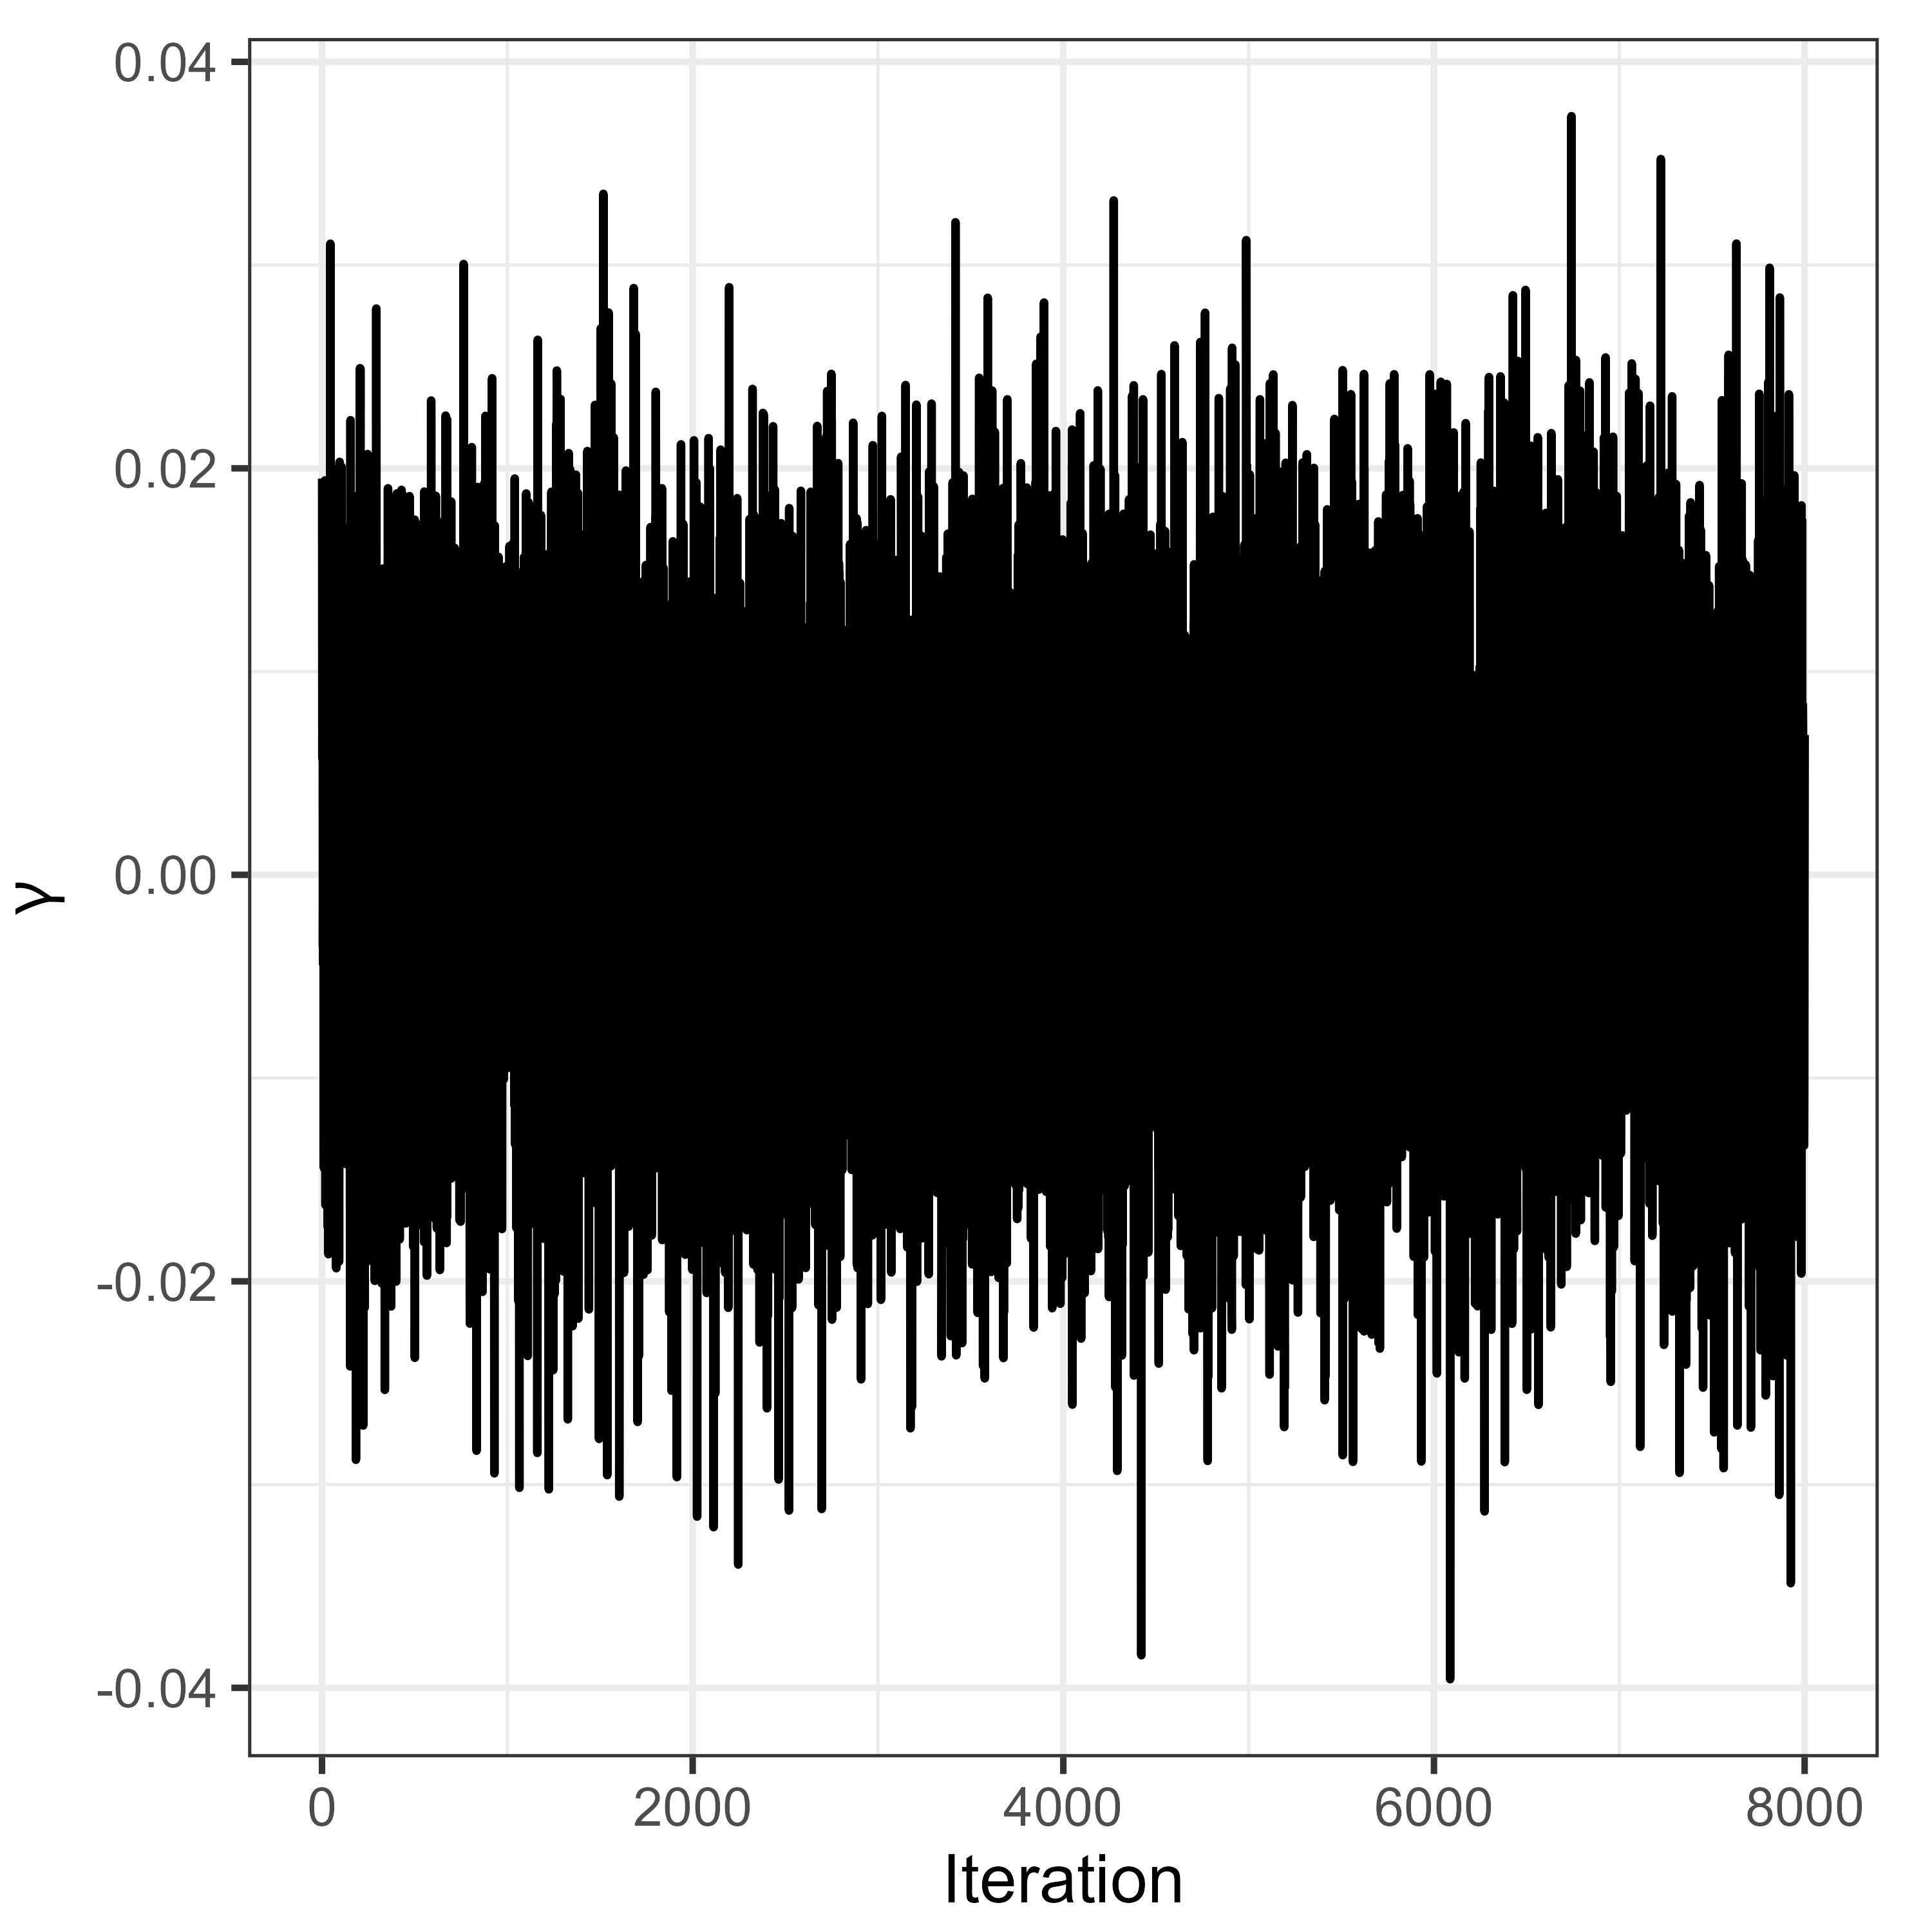
\includegraphics[width=0.45\textwidth]{../figures/simulation/trace_gamma.png}
    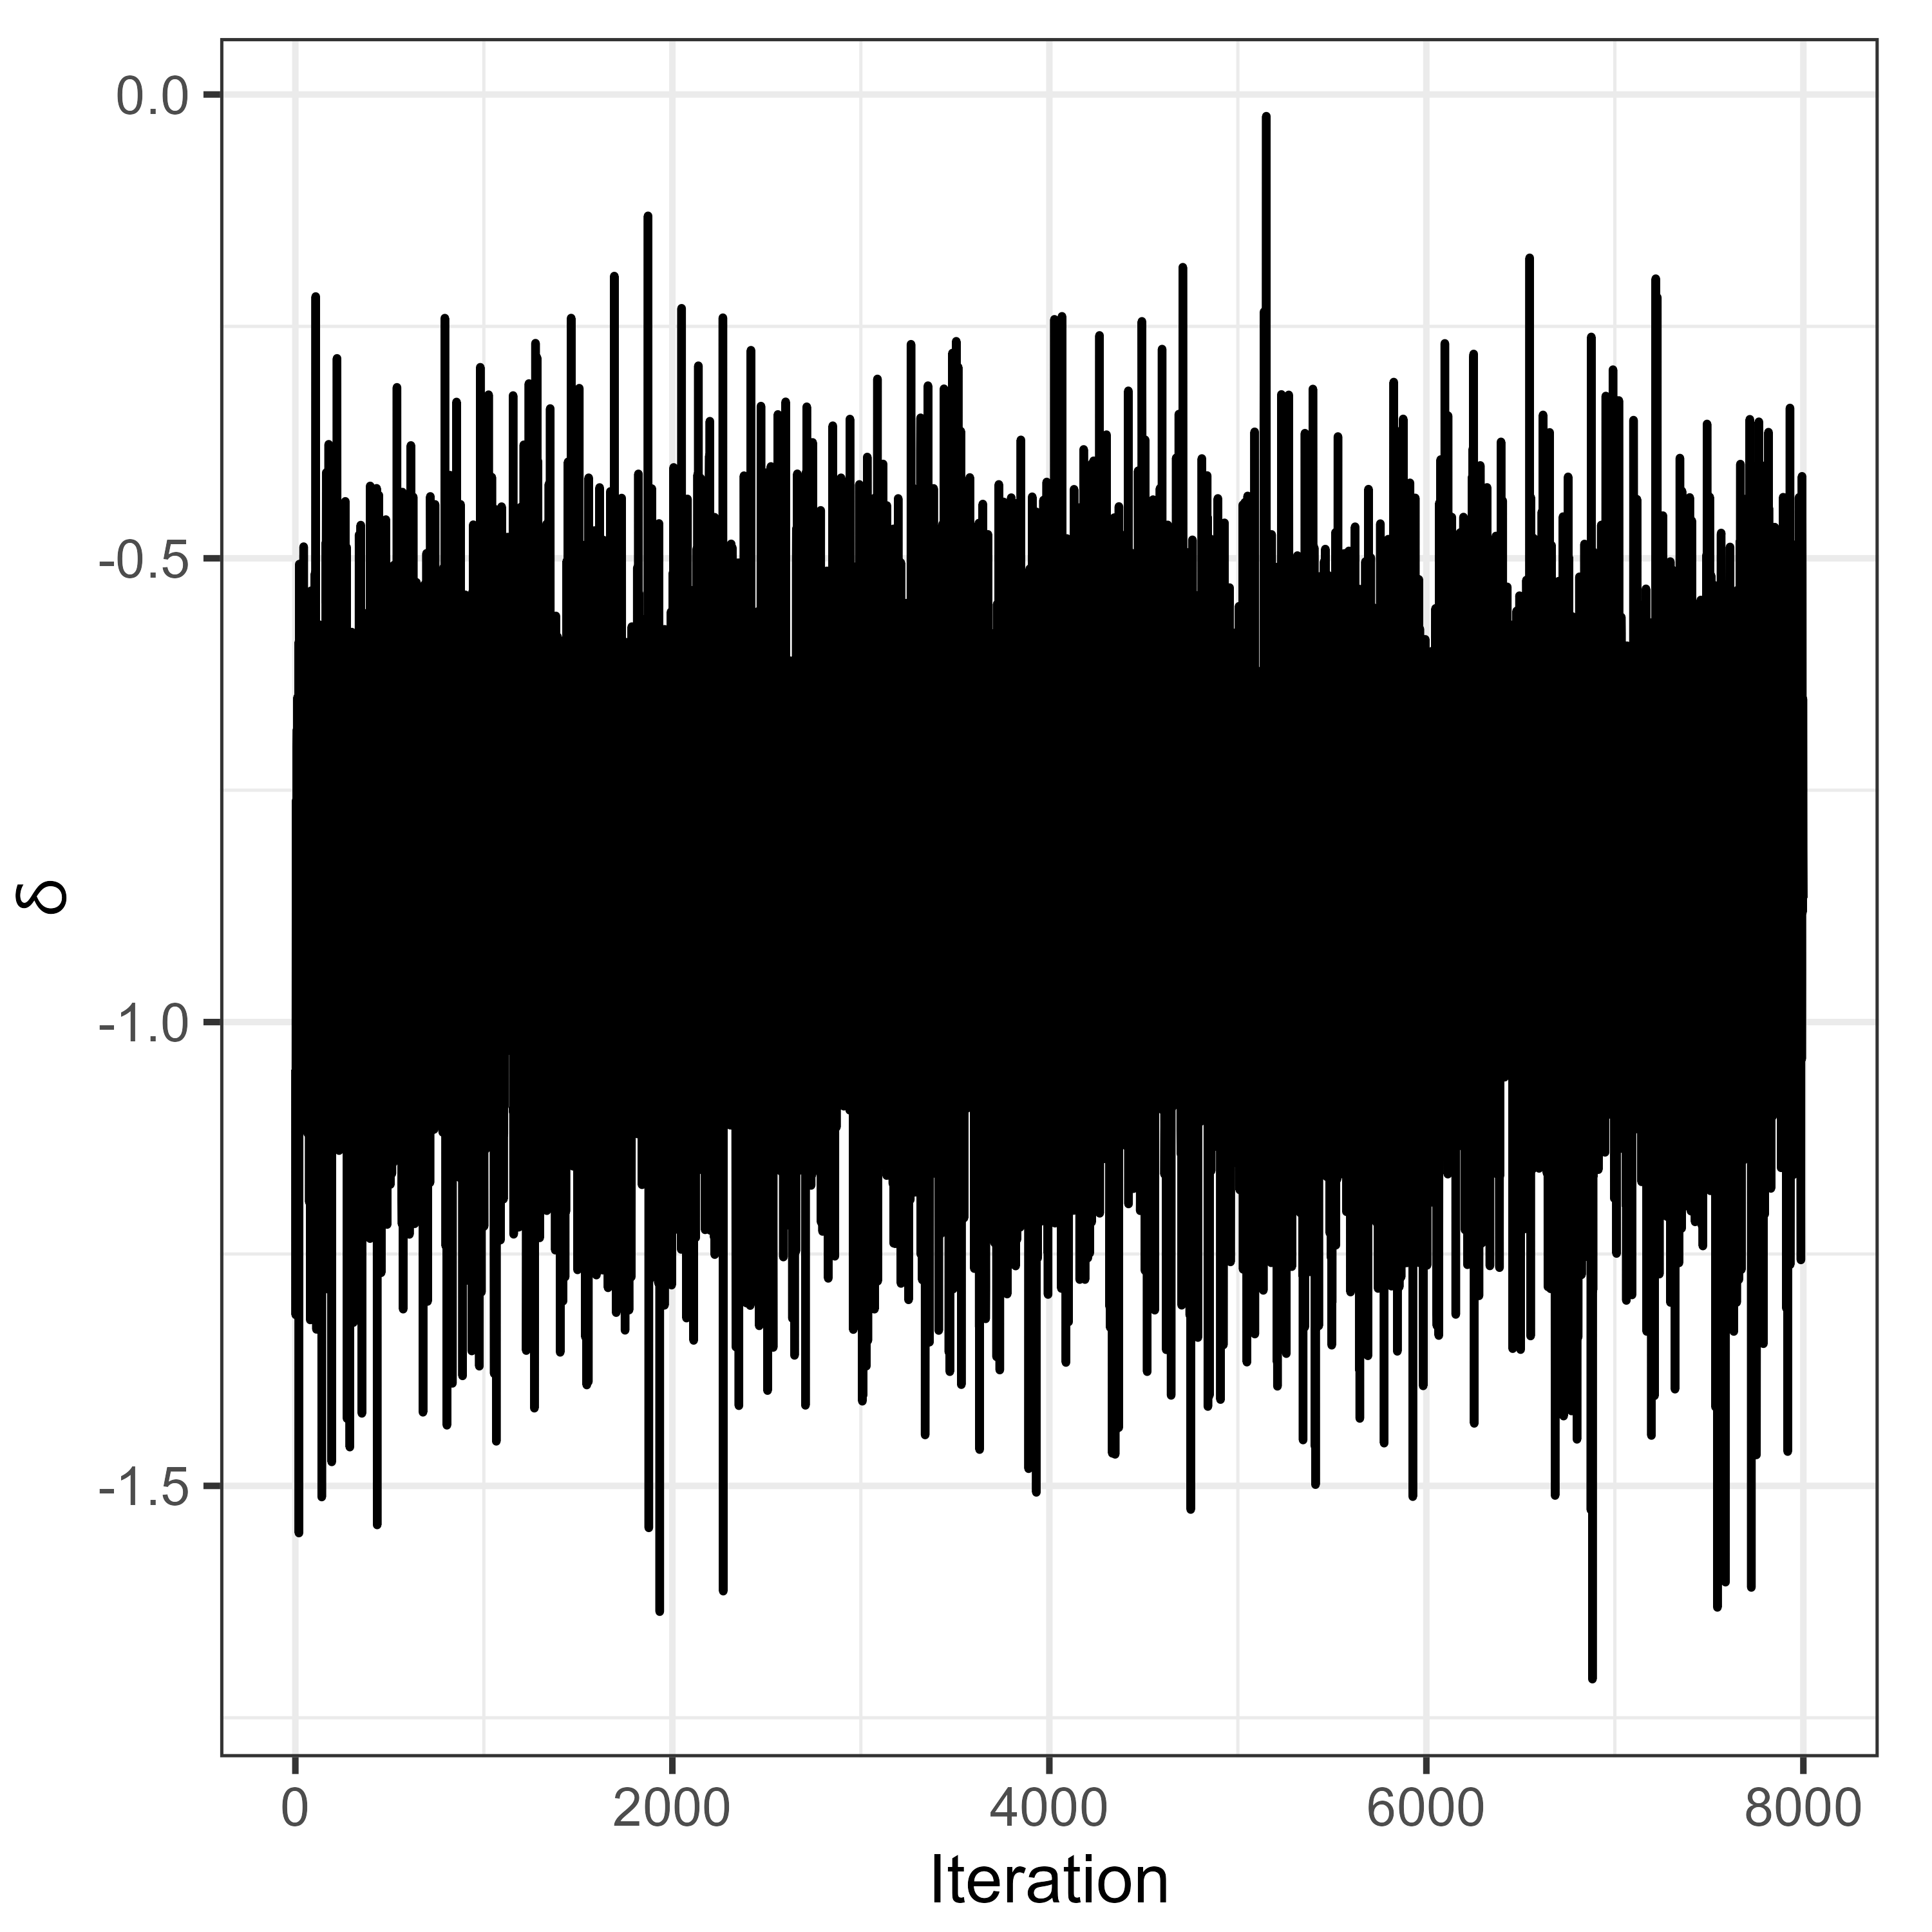
\includegraphics[width=0.45\textwidth]{../figures/simulation/trace_delta.png}
    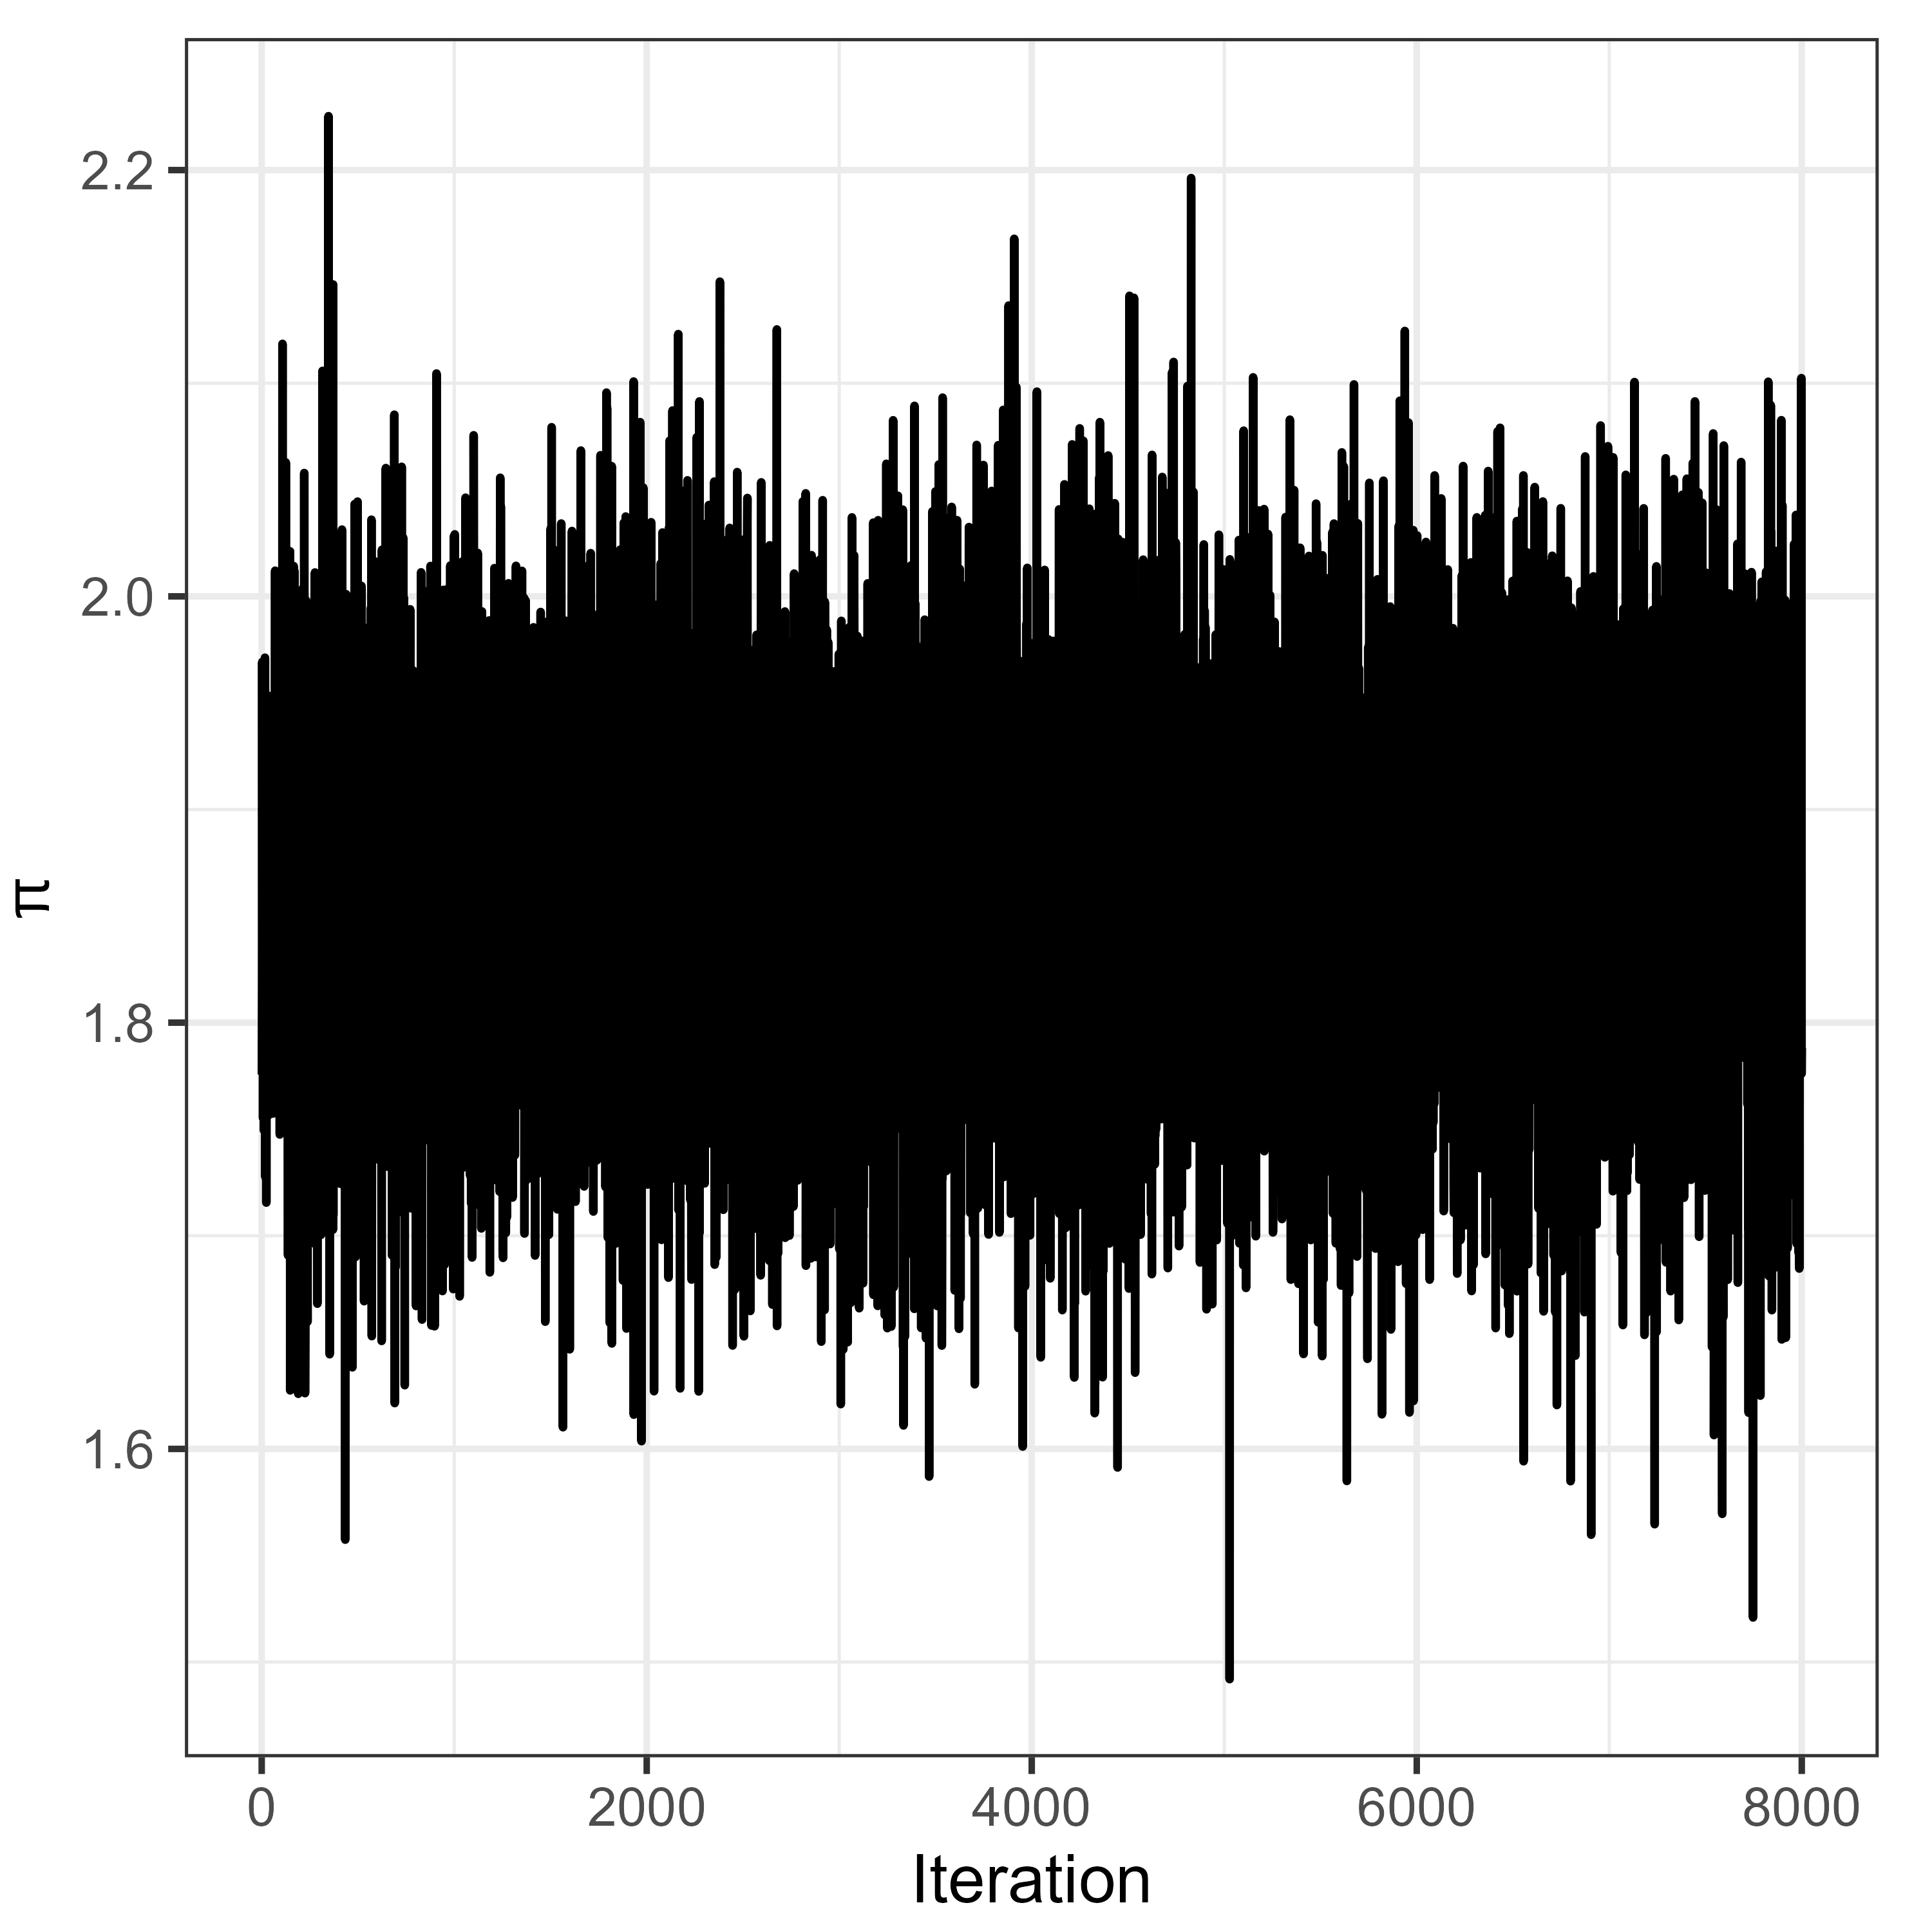
\includegraphics[width=0.45\textwidth]{../figures/simulation/trace_pi.png}
    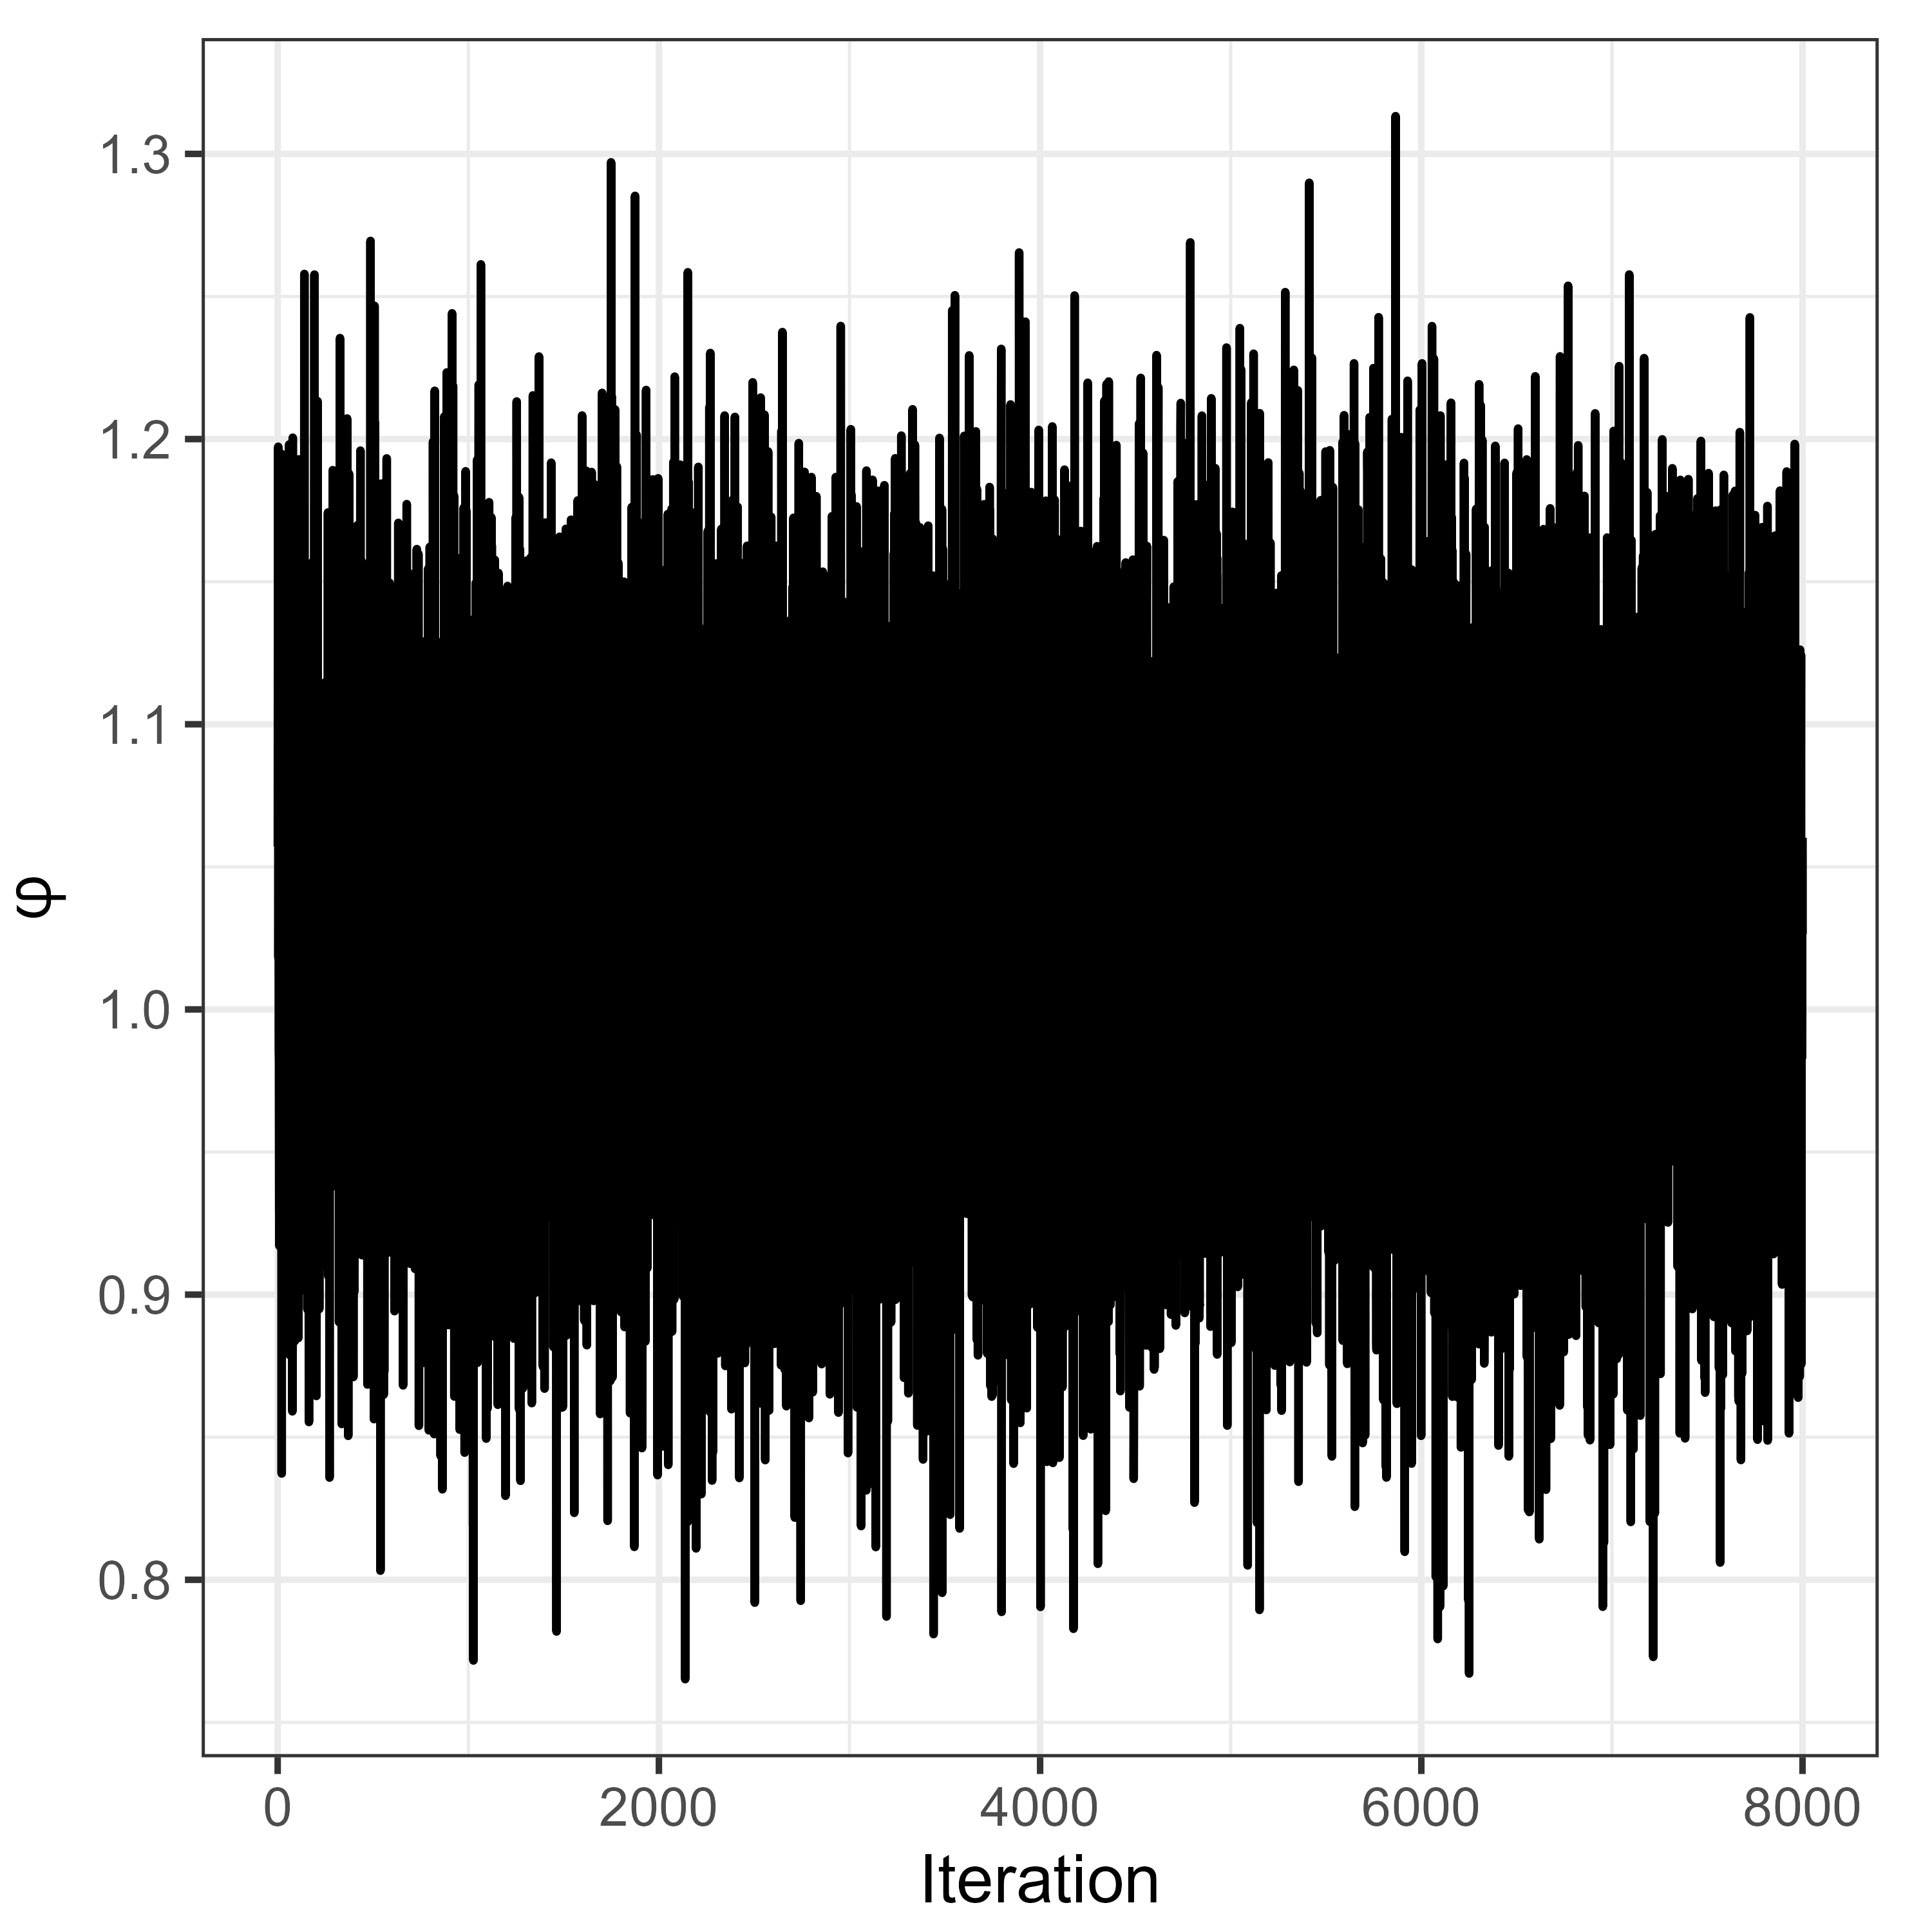
\includegraphics[width=0.45\textwidth]{../figures/simulation/trace_phi.png}
    \caption{Traceplots of $\gamma$, $\delta$, $\pi$, and $\phi$ --- Simulation Study}
    \label{fig:posterior_traceplots_2}
    \end{figure}
    
\begin{figure}[H]
    \centering
    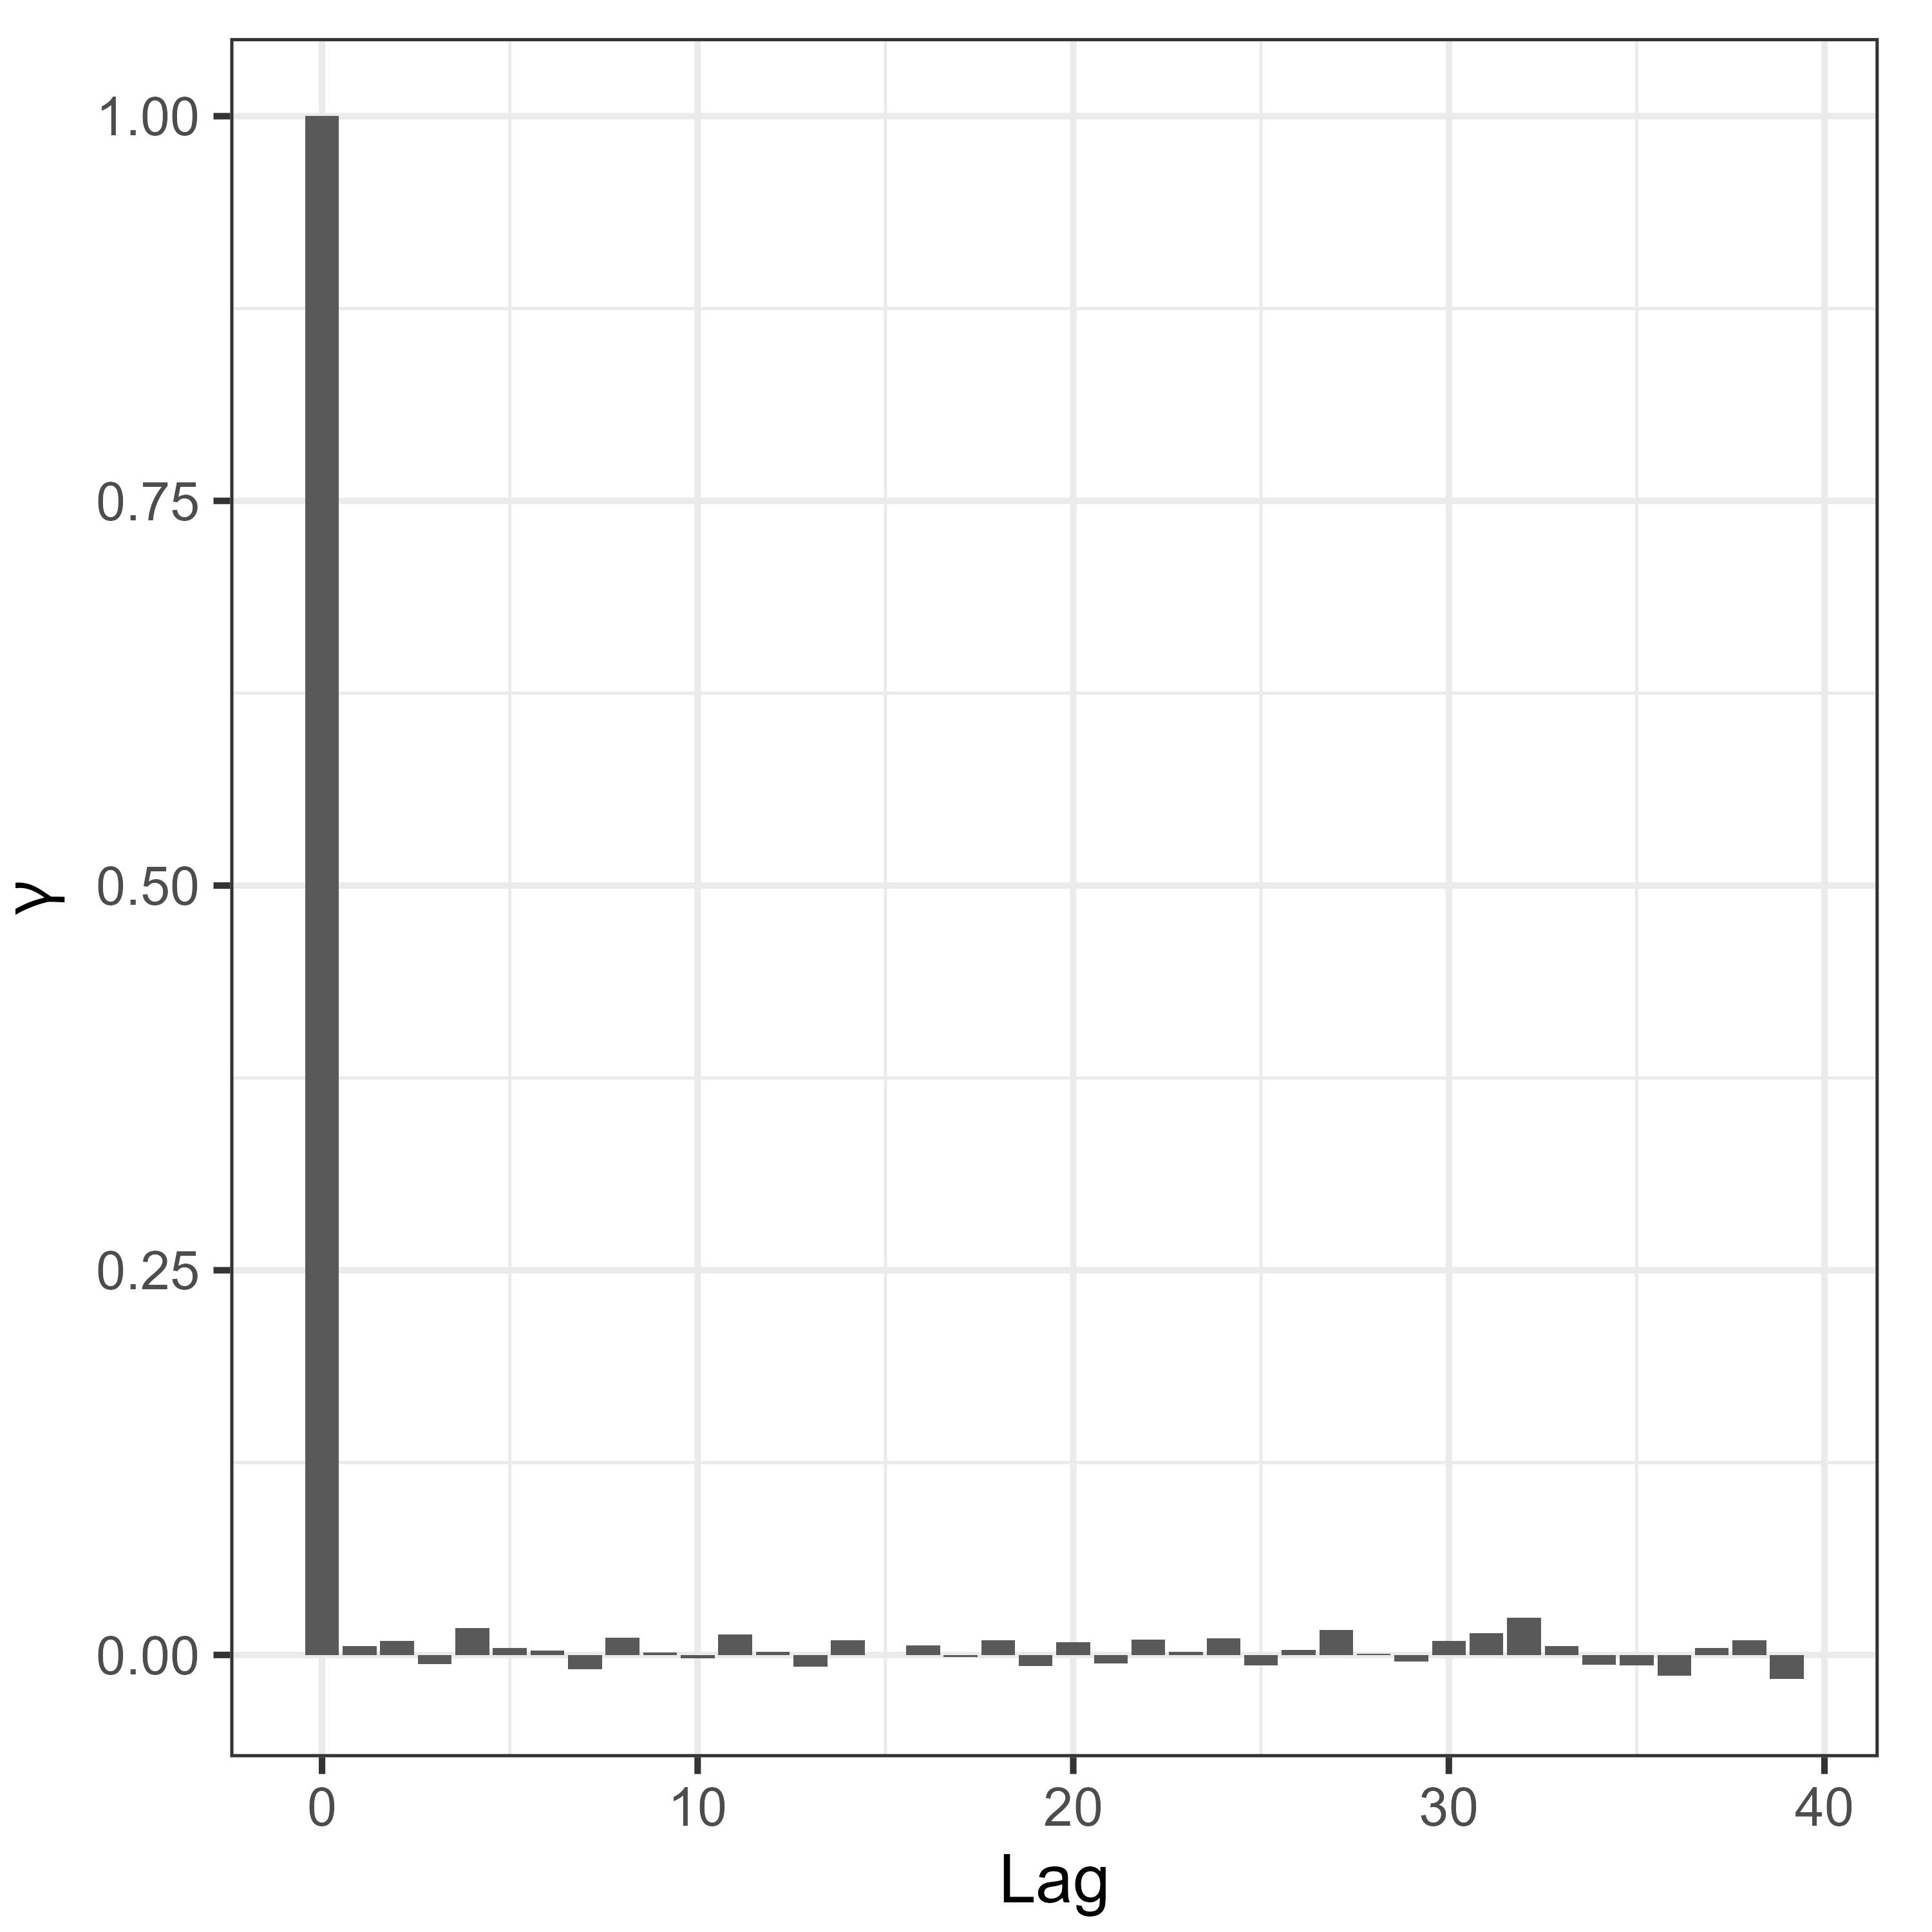
\includegraphics[width=0.45\textwidth]{../figures/simulation/acf_gamma.png}
    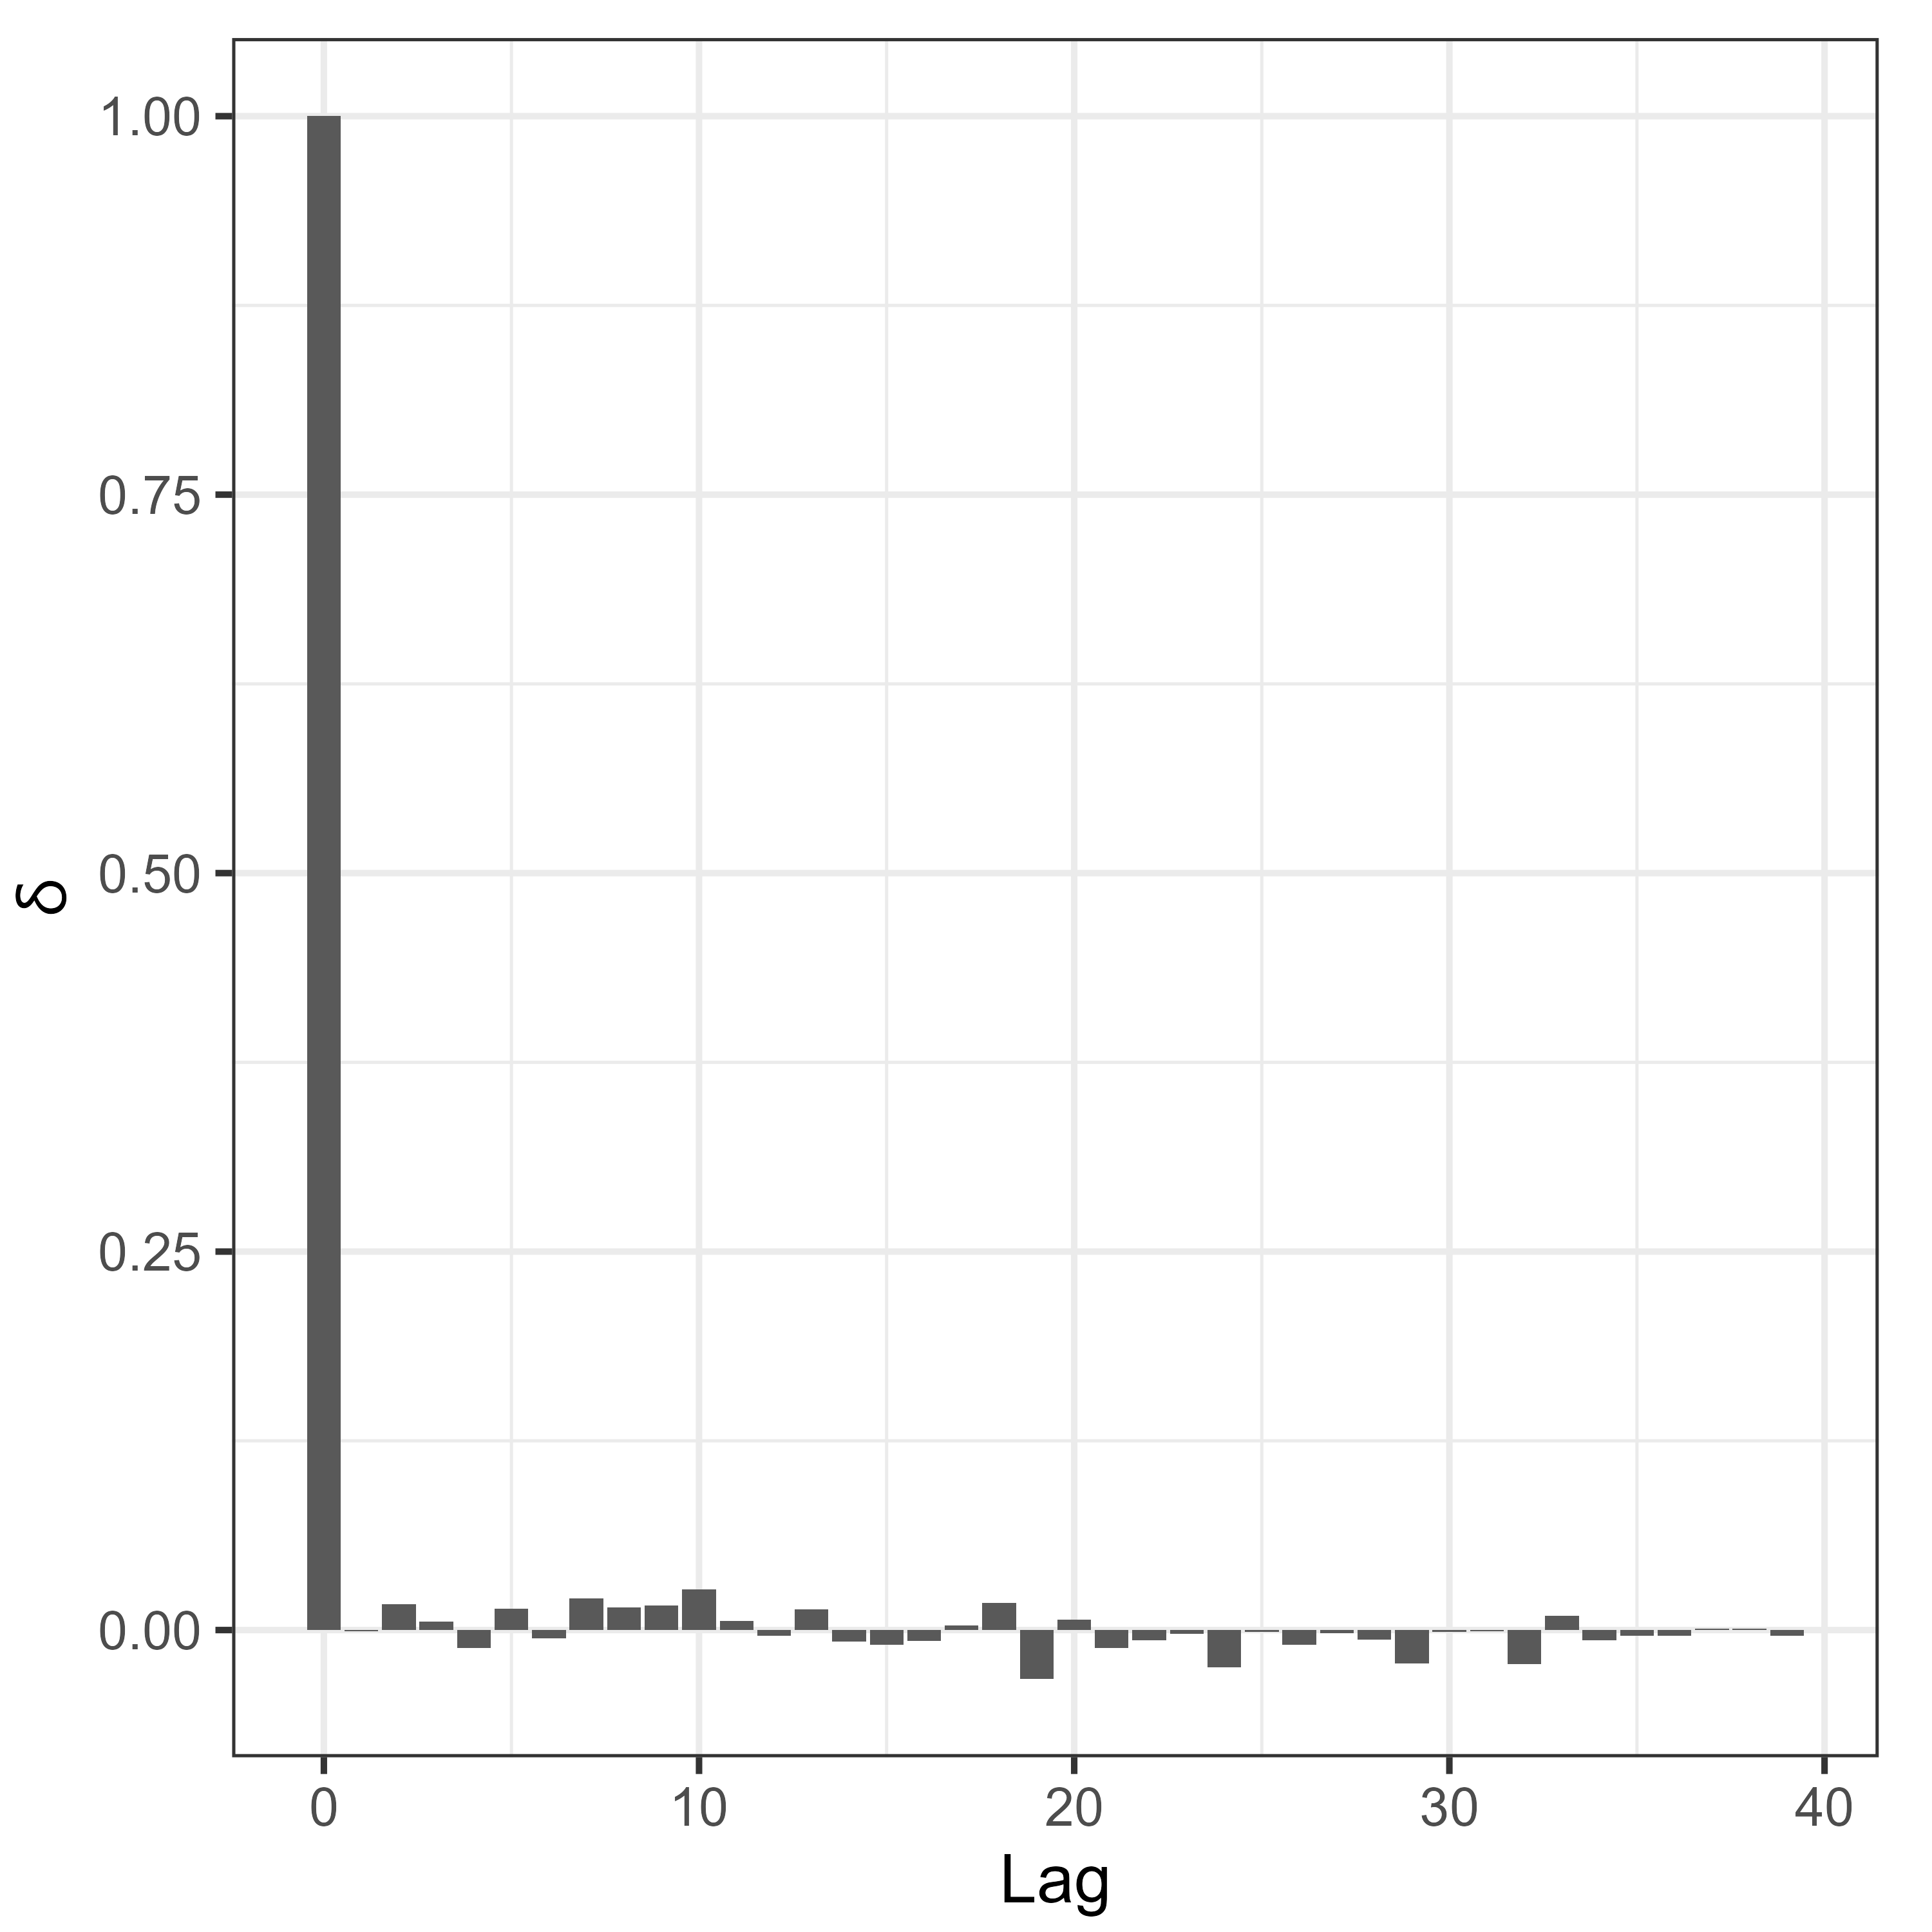
\includegraphics[width=0.45\textwidth]{../figures/simulation/acf_delta.png}
    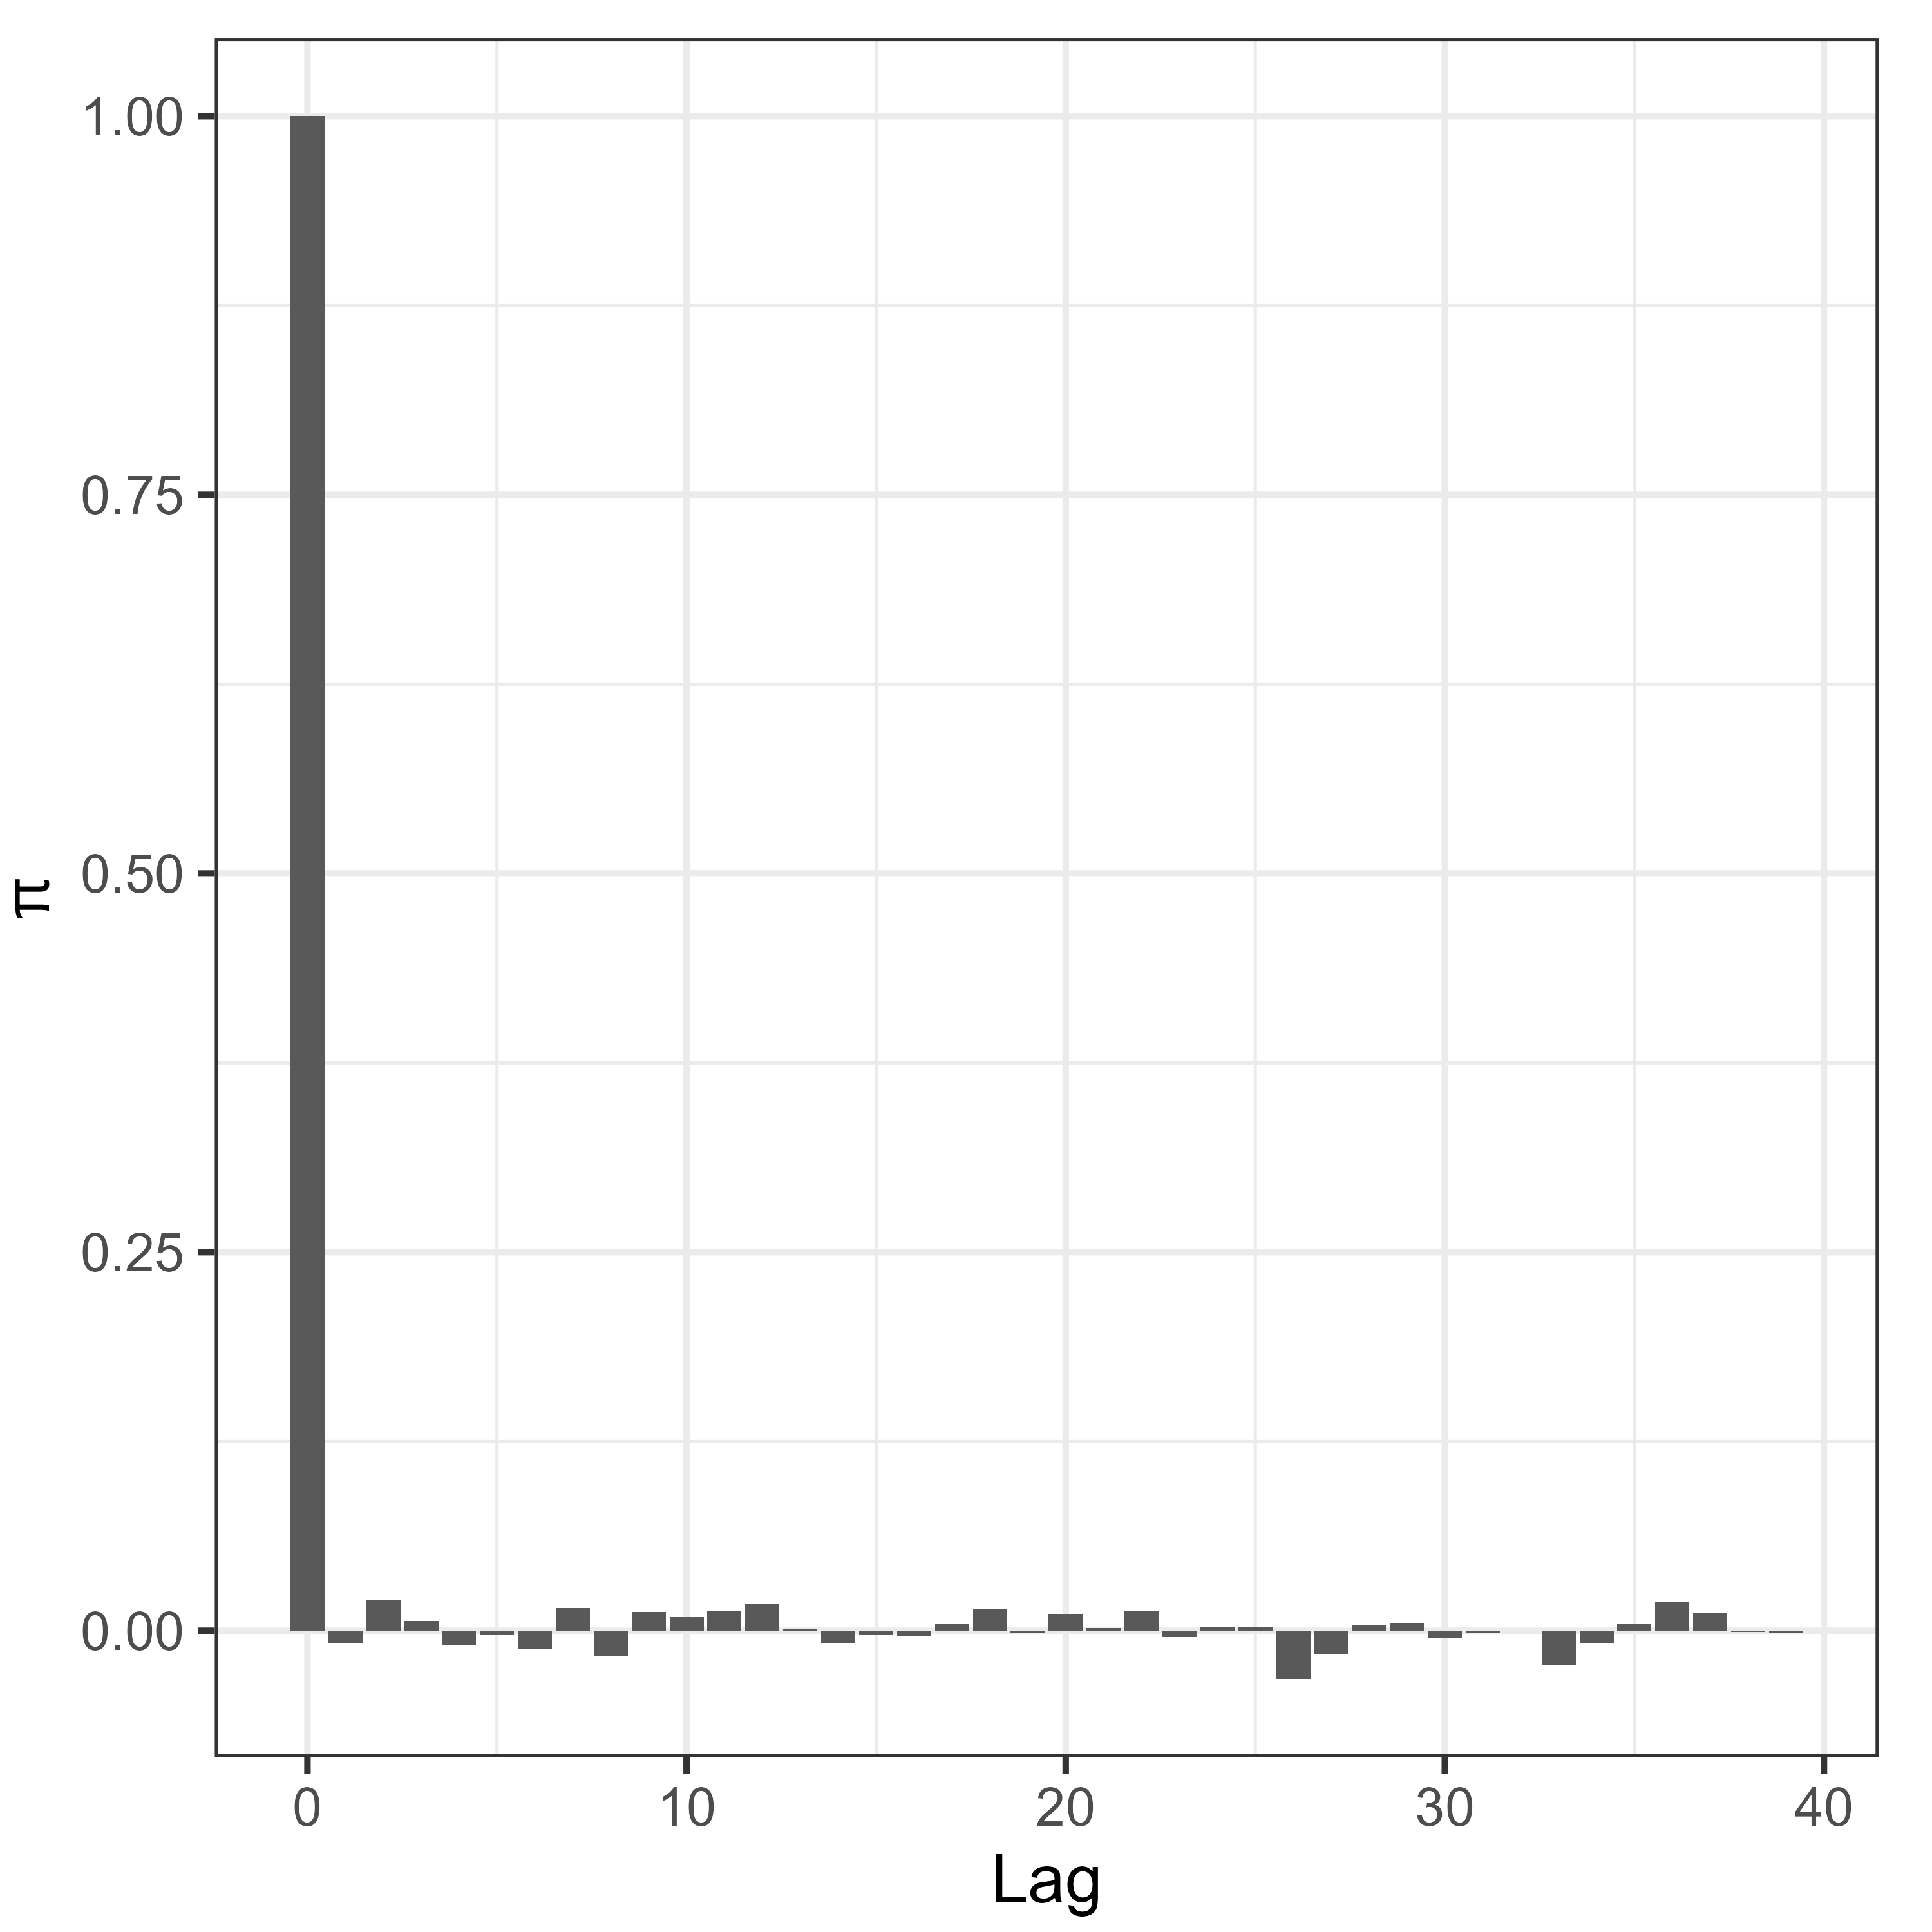
\includegraphics[width=0.45\textwidth]{../figures/simulation/acf_pi.png}
    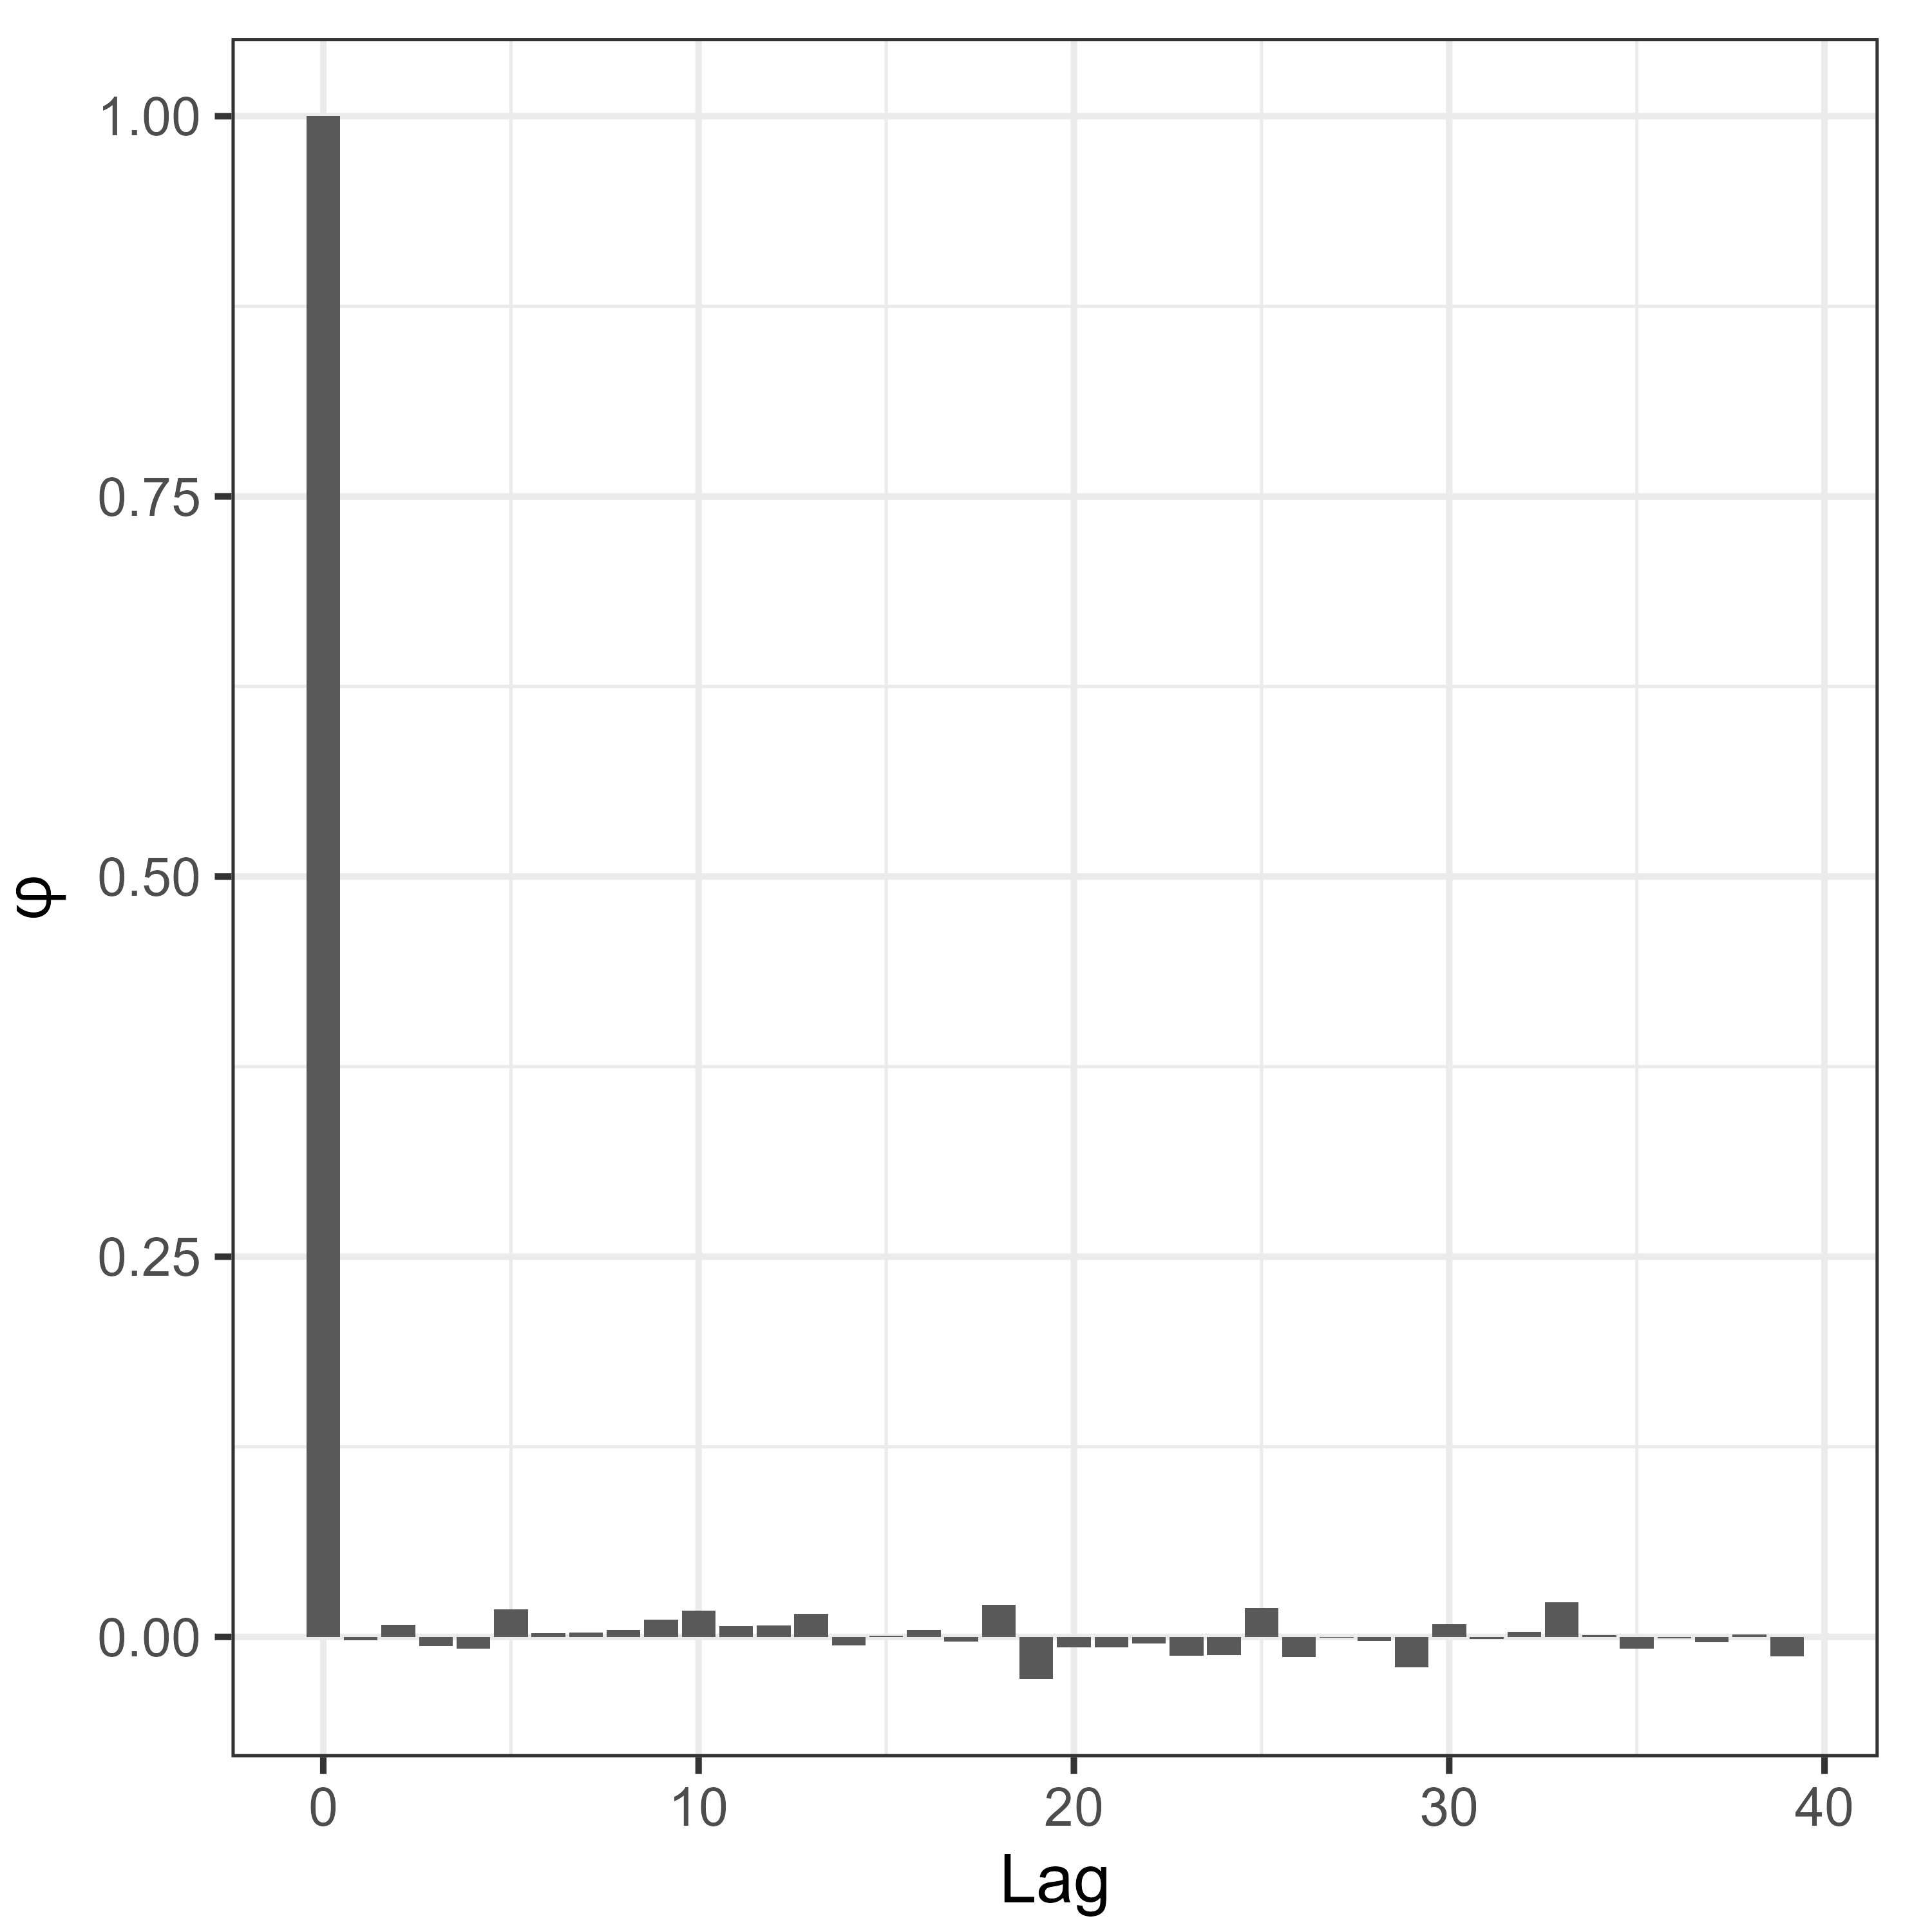
\includegraphics[width=0.45\textwidth]{../figures/simulation/acf_phi.png}
    \caption{Autocorrelation of $\gamma$, $\delta$, $\pi$, and $\phi$ --- Simulation Study}
    \label{fig:posterior_autocorrelation_2}
\end{figure}    
    
\begin{figure}[H]
\centering
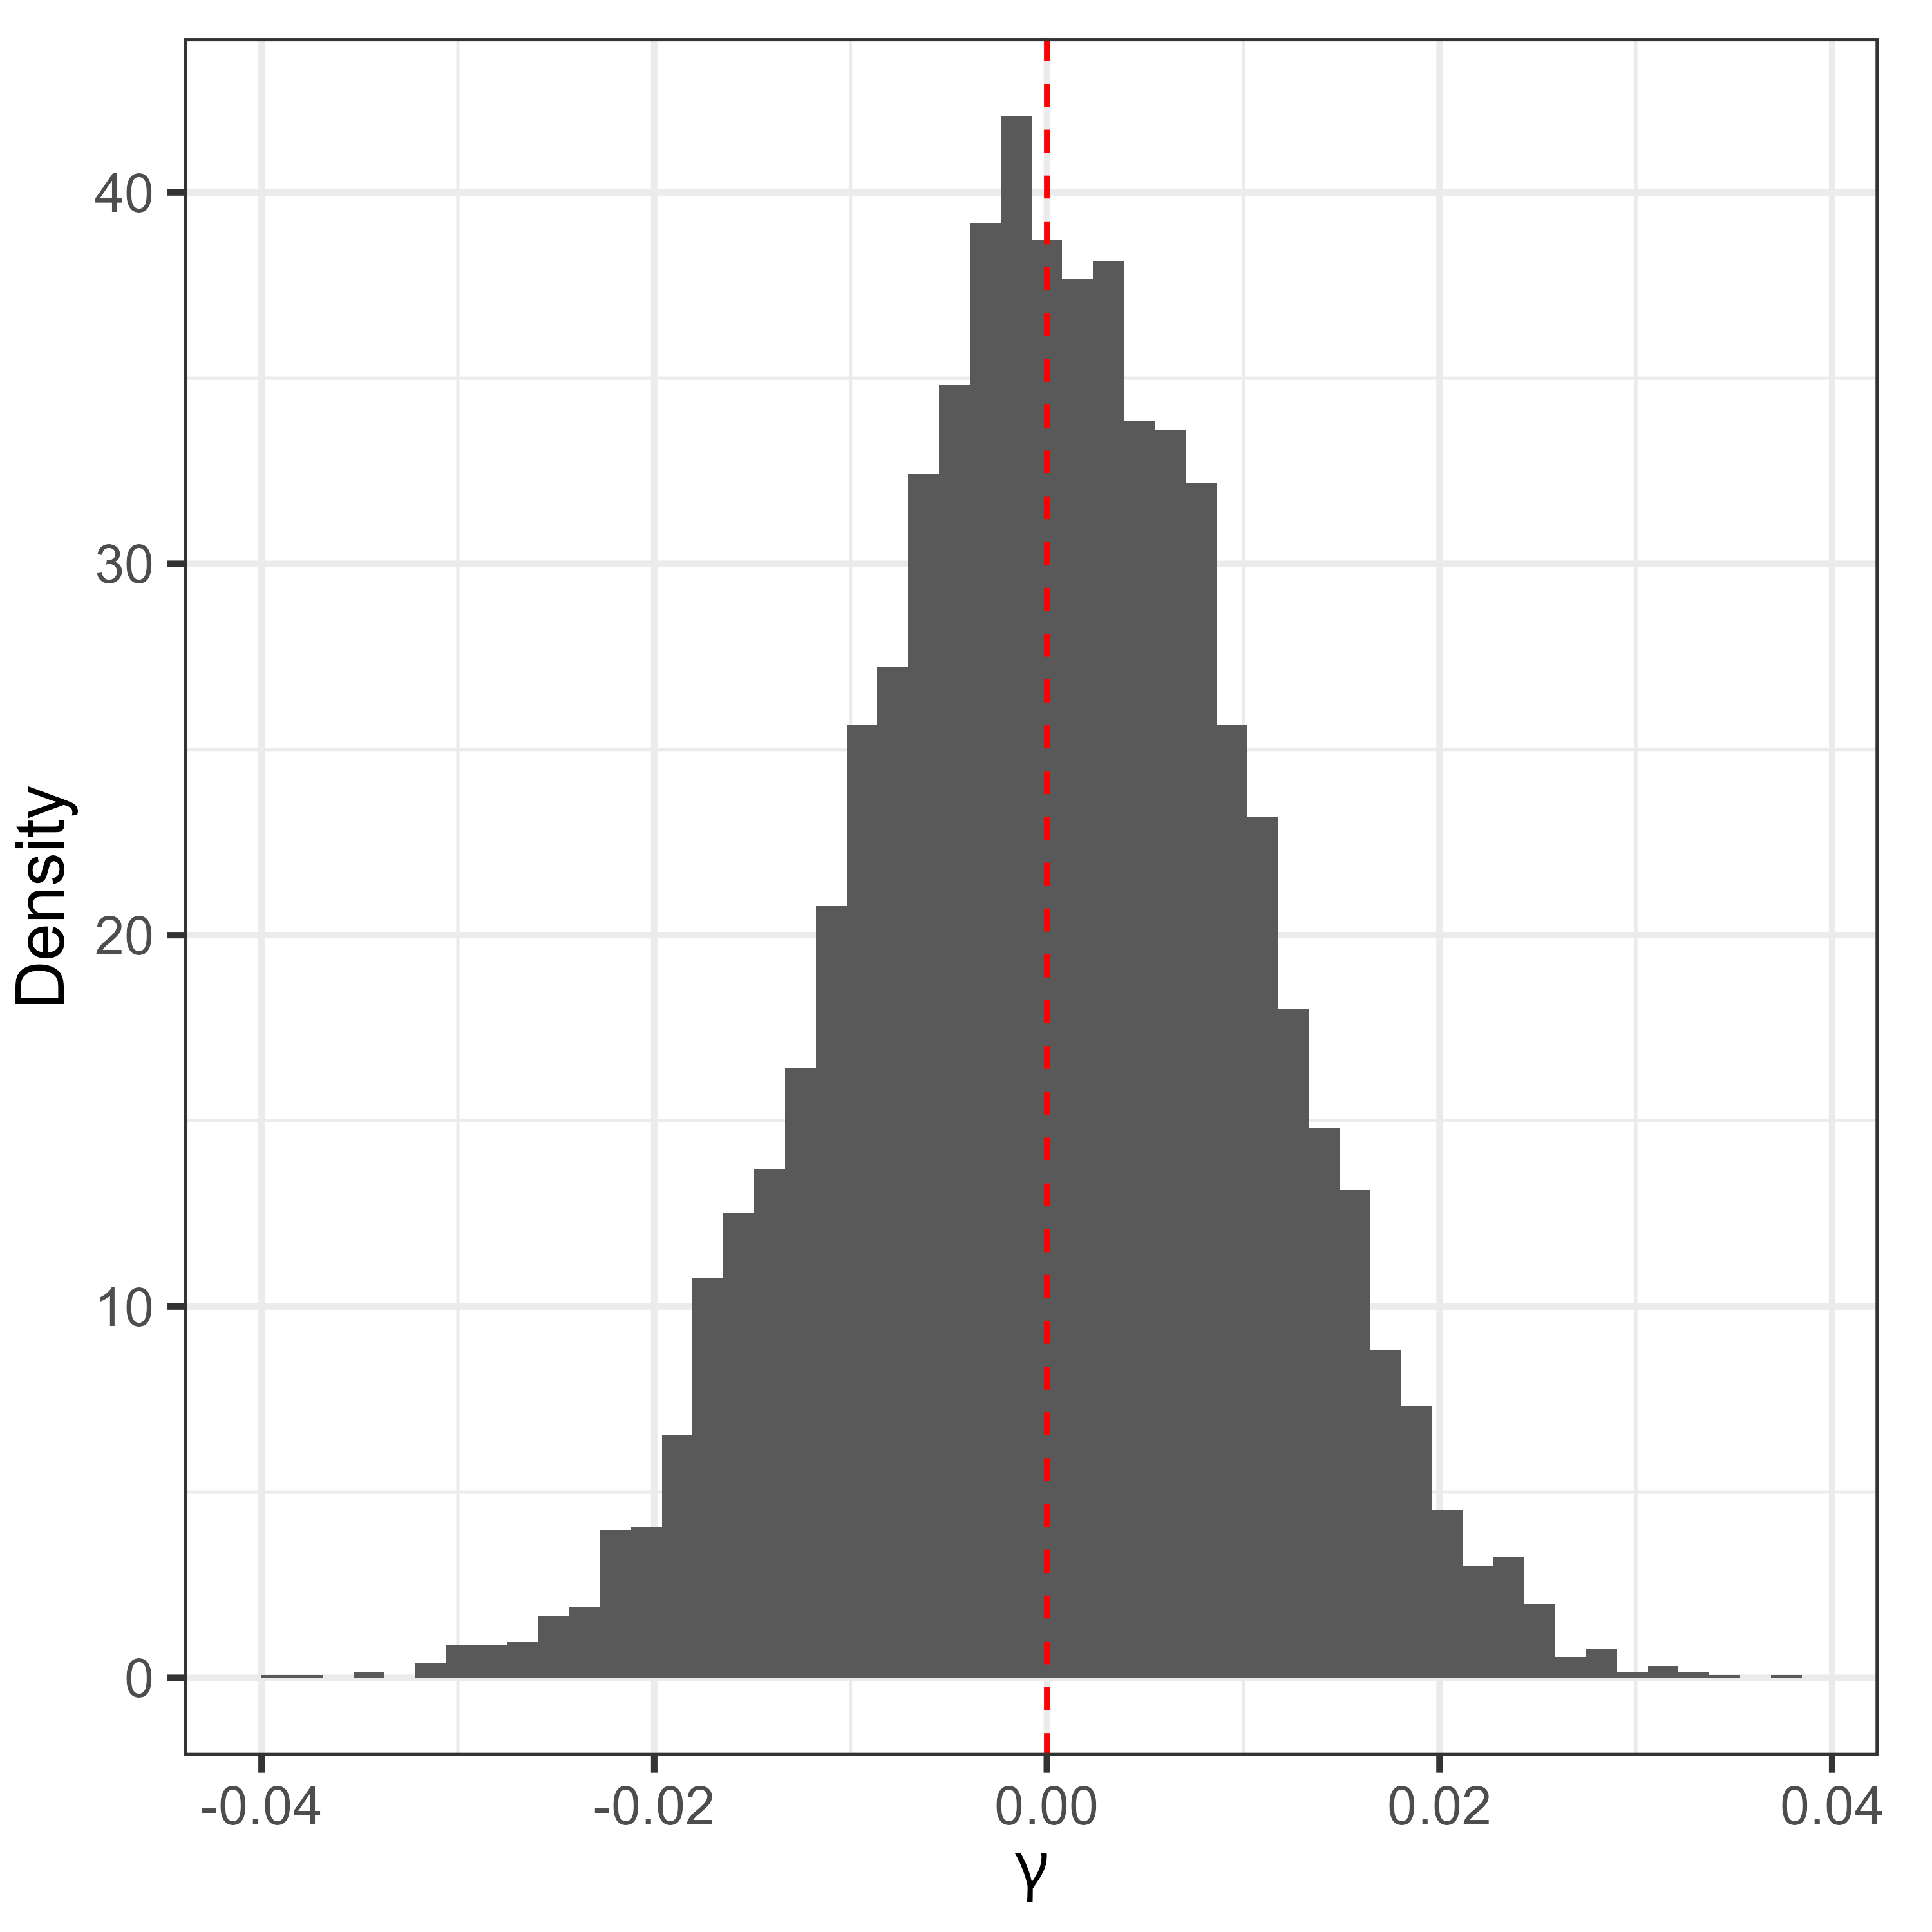
\includegraphics[width=0.45\textwidth]{../figures/simulation/hist_gamma.png}
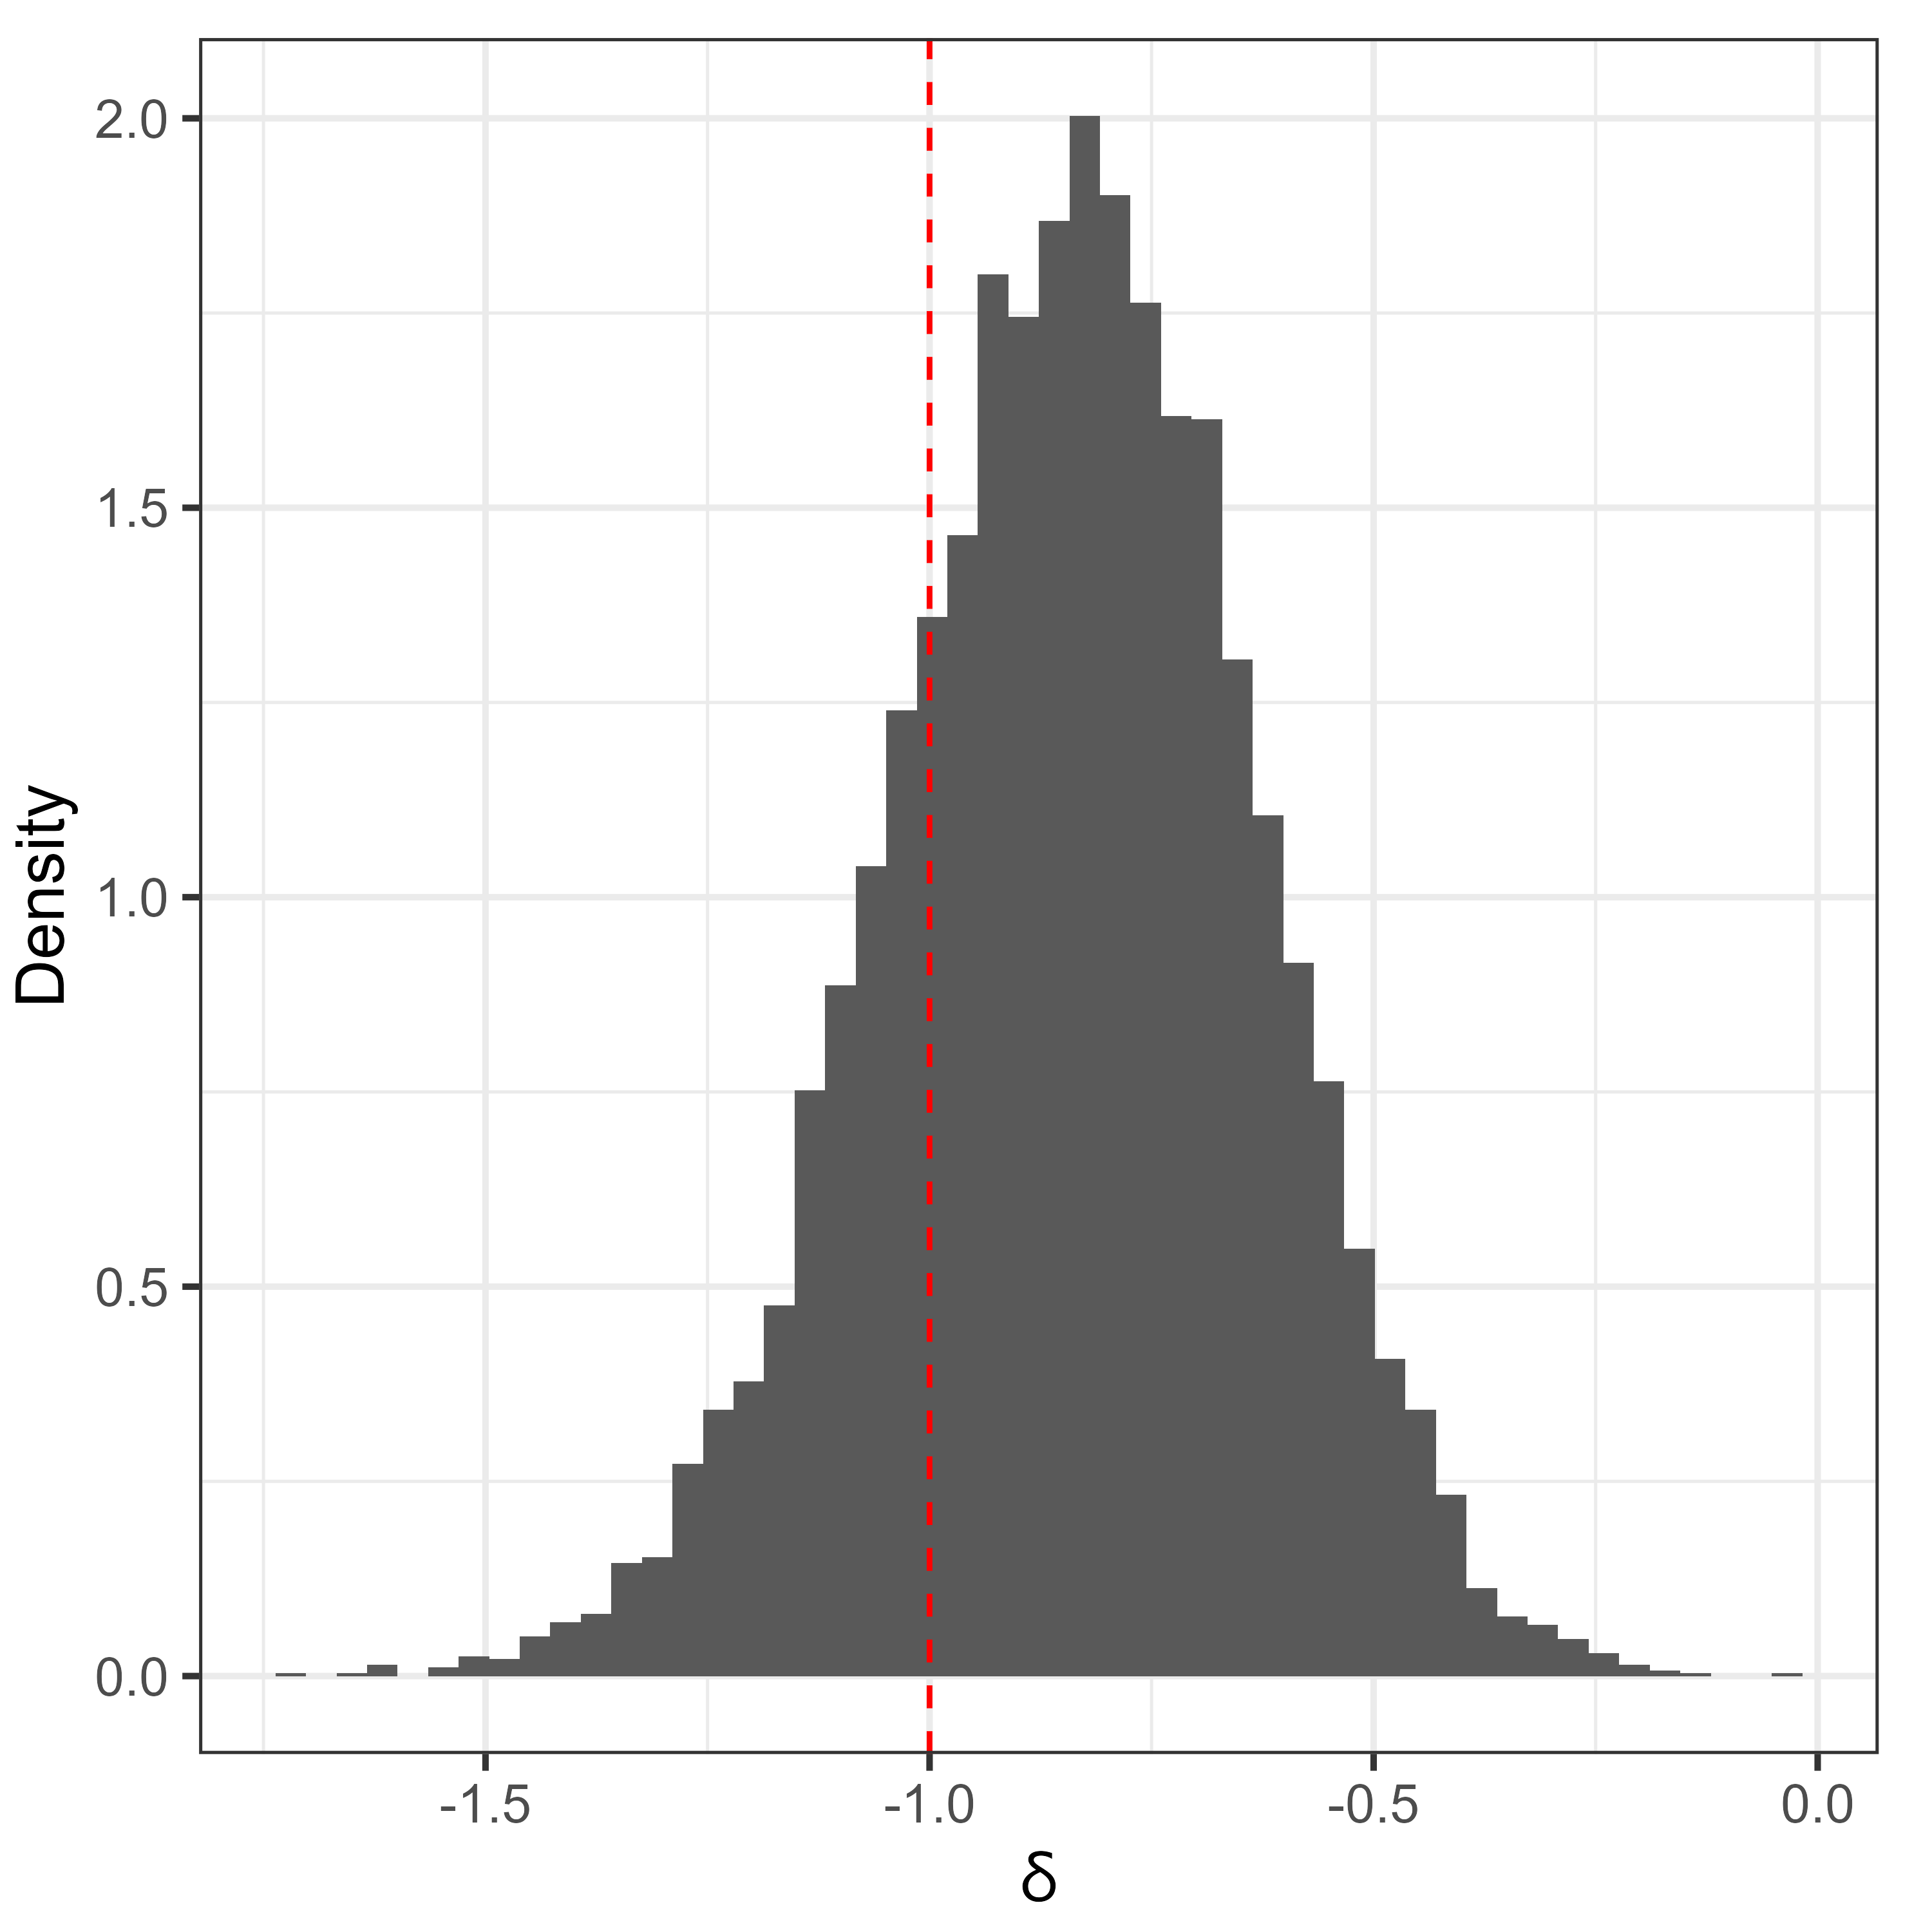
\includegraphics[width=0.45\textwidth]{../figures/simulation/hist_delta.png}
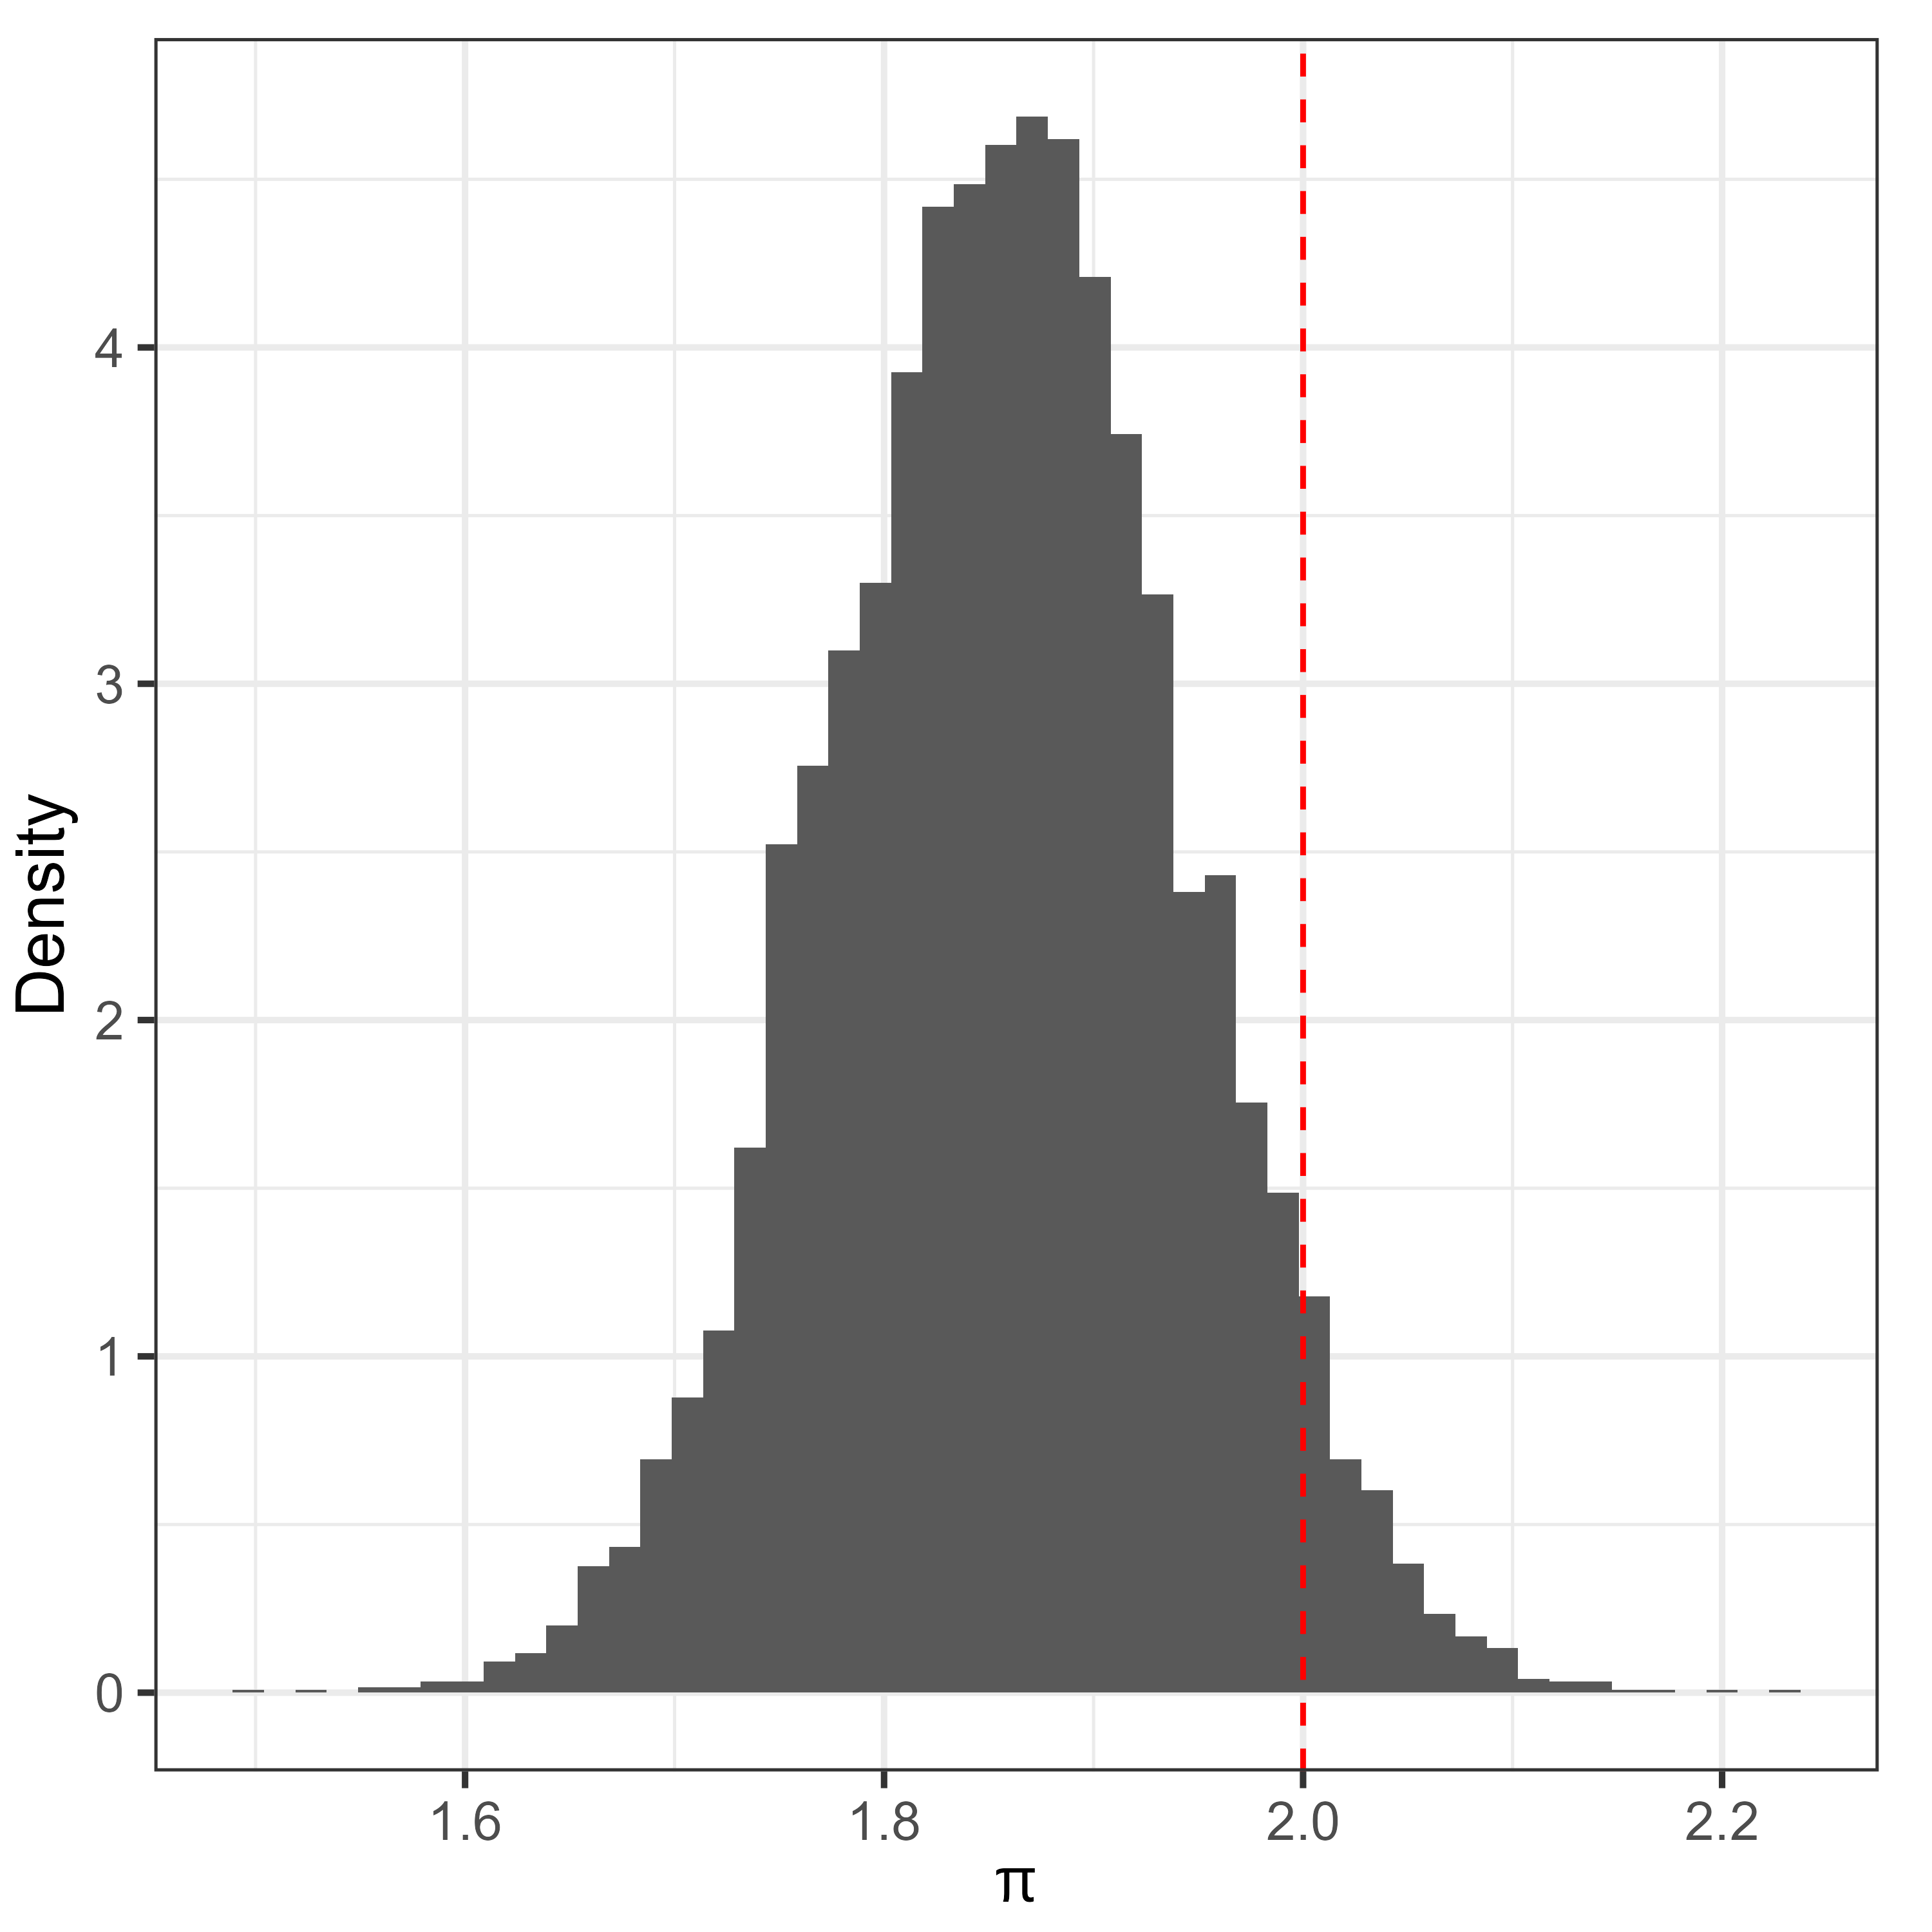
\includegraphics[width=0.45\textwidth]{../figures/simulation/hist_pi.png}
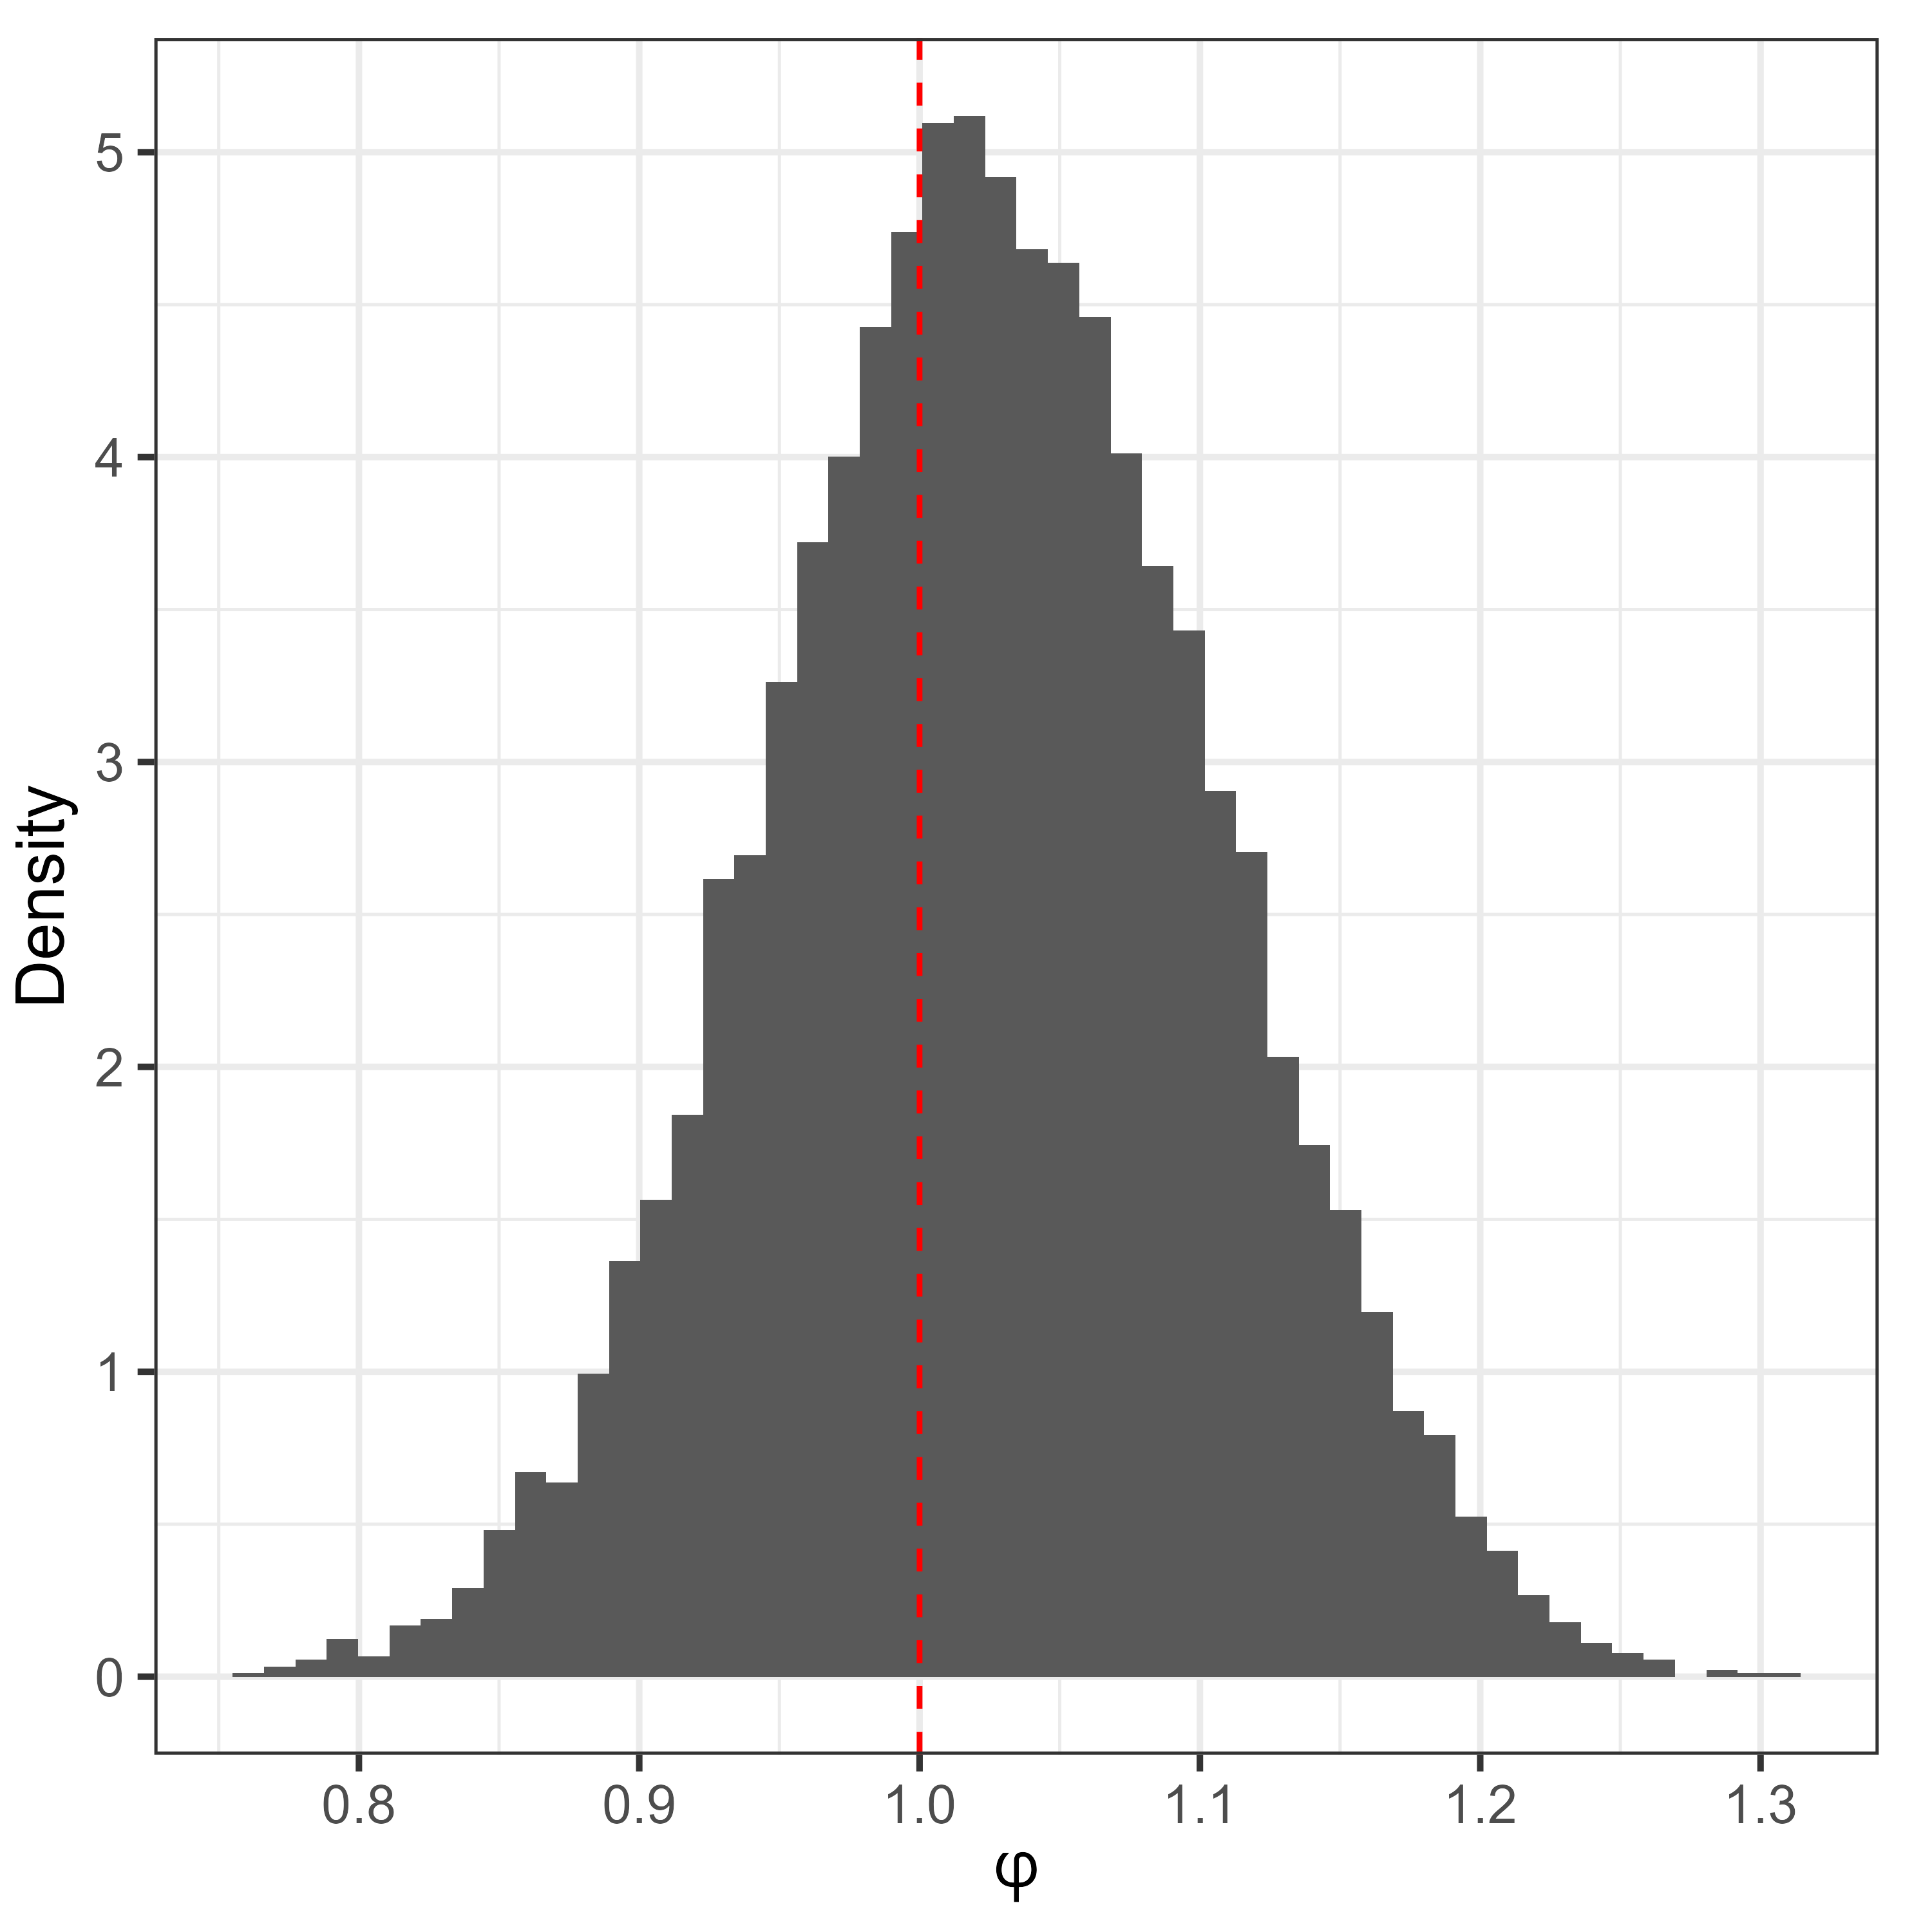
\includegraphics[width=0.45\textwidth]{../figures/simulation/hist_phi.png}
\caption{Posterior Distributions of $\gamma$, $\delta$, $\pi$, and $\phi$ --- Simulation Study}
\label{fig:posterior_distributions_2}
\end{figure}

This indicates that the Gibbs sampler is able to recover the true parameters of the model, even with a small sample size. As we parametrize the model with easy to sample priors and our Markov chain is well-behaved with a low autocorrelation, each additional sample is effectively independent. This can be seen in the Effective Sample Size (ESS) in Table \ref{tab:simulation_results}, which is close to the total number of samples, including for the $\beta$ variable a larger than 10,000 ESS as the autocorrelation for this variable is negative for some lags.

\subsection{Second Study}

For the second simulation exercise, we run three additional comparative analyses to assess the performance of the Bayesian plausibly exogenous model under different conditions. Specifically, we compare:

\begin{itemize}
    \item \textbf{Weak vs. Strong Instruments:} We vary the strength of the instrument by incorporating different noise levels in the data. 
    \item \textbf{Narrow vs. Wide Priors:} We compare results obtained under highly informative priors (small prior variance for $\gamma$) against results under weakly informative priors (large prior variance).
    \item \textbf{Valid vs. Invalid Instrument:} We contrast cases where the true value of $\gamma$ is zero (valid instrument) and where $\gamma$ is nonzero (invalid instrument).
\end{itemize}

For each scenario, we run the Gibbs sampler for $10{,}000$ iterations, discarding the first $5{,}000$ as burn-in. The posterior summary statistics for each setting are reported in Table \ref{tab:models}.


% Table created by stargazer v.5.2.3 by Marek Hlavac, Social Policy Institute. E-mail: marek.hlavac at gmail.com
% Date and time: Mon, Apr 28, 2025 - 11:48:21 PM
\begin{table}[!htbp] \centering 
  \caption{Simulation Results} 
  \label{tab:models} 
\begin{tabular}{@{\extracolsep{5pt}} ccccc} 
\\[-1.8ex]\hline 
\hline \\[-1.8ex] 
 & Mean & Standard Deviation & Lower CI & Upper CI \\ 
\hline \\[-1.8ex] 
Baseline & $2.03$ & $0.09$ & $1.85$ & $2.23$ \\ 
Weak Instrument & $0.16$ & $1.93$ & $$-$3.66$ & $4.20$ \\ 
Uncertain Instrument & $1.94$ & $0.52$ & $0.93$ & $2.97$ \\ 
Invalid Instrument & $7.04$ & $0.36$ & $6.37$ & $7.76$ \\ 
\hline \\[-1.8ex] 
\end{tabular} 
\end{table} 


\subsection{Third Study}
In this third simulation exercise, we conduct a sensitivity analysis by jointly varying the prior variance and the true value of $\gamma$, while examining the resulting posterior estimates of $\beta$. We focus initially on the case where the true $\gamma$ is fixed at $0$, and analyze how $\widehat{\beta}$ responds to different levels of prior informativeness regarding $\gamma$.

If the prior variance on $\gamma$ is set too small, the Bayesian procedure behaves similarly to imposing the sharp exclusion restriction $\gamma = 0$. In such cases, if $\gamma$ is not exactly zero, the estimator can suffer from omitted variable bias. Conversely, if the prior variance is set too large, the prior becomes weakly informative, approaching the behavior of ordinary least squares (OLS). In this limit, the estimator may lose precision and significance, because it allows for large direct effects of the instrument.

This exercise parallels the idea of \emph{sensitivity analysis}, as discussed in \cite{cinelliMakingSenseSensitivity2020}, where the robustness of causal conclusions to violations of identifying assumptions is systematically explored. In their paper, they propose a method to assess the sensitivity of causal conclusions to potential omitted variable bias. In our case, we are interested in the sensitivity of the posterior estimates of $\beta$ to the prior variance of $\gamma$.

The procedure follows the steps below:
\begin{itemize}
    \item Fix the true value of $\gamma$ (initially set to 0).
    \item Vary the prior variance of $\gamma$ across a wide grid of values, from highly informative (small variance) to weakly informative (large variance).
    \item For each specification, run the Gibbs sampler and record the posterior mean and credible interval for $\beta$.
\end{itemize}

The results are presented in Figure \ref{fig:sensitivity_analysis_beta}, which plots the posterior mean and credible intervals of $\beta$ against the log of the prior variance of $\gamma$.

\begin{figure}[H]
\centering
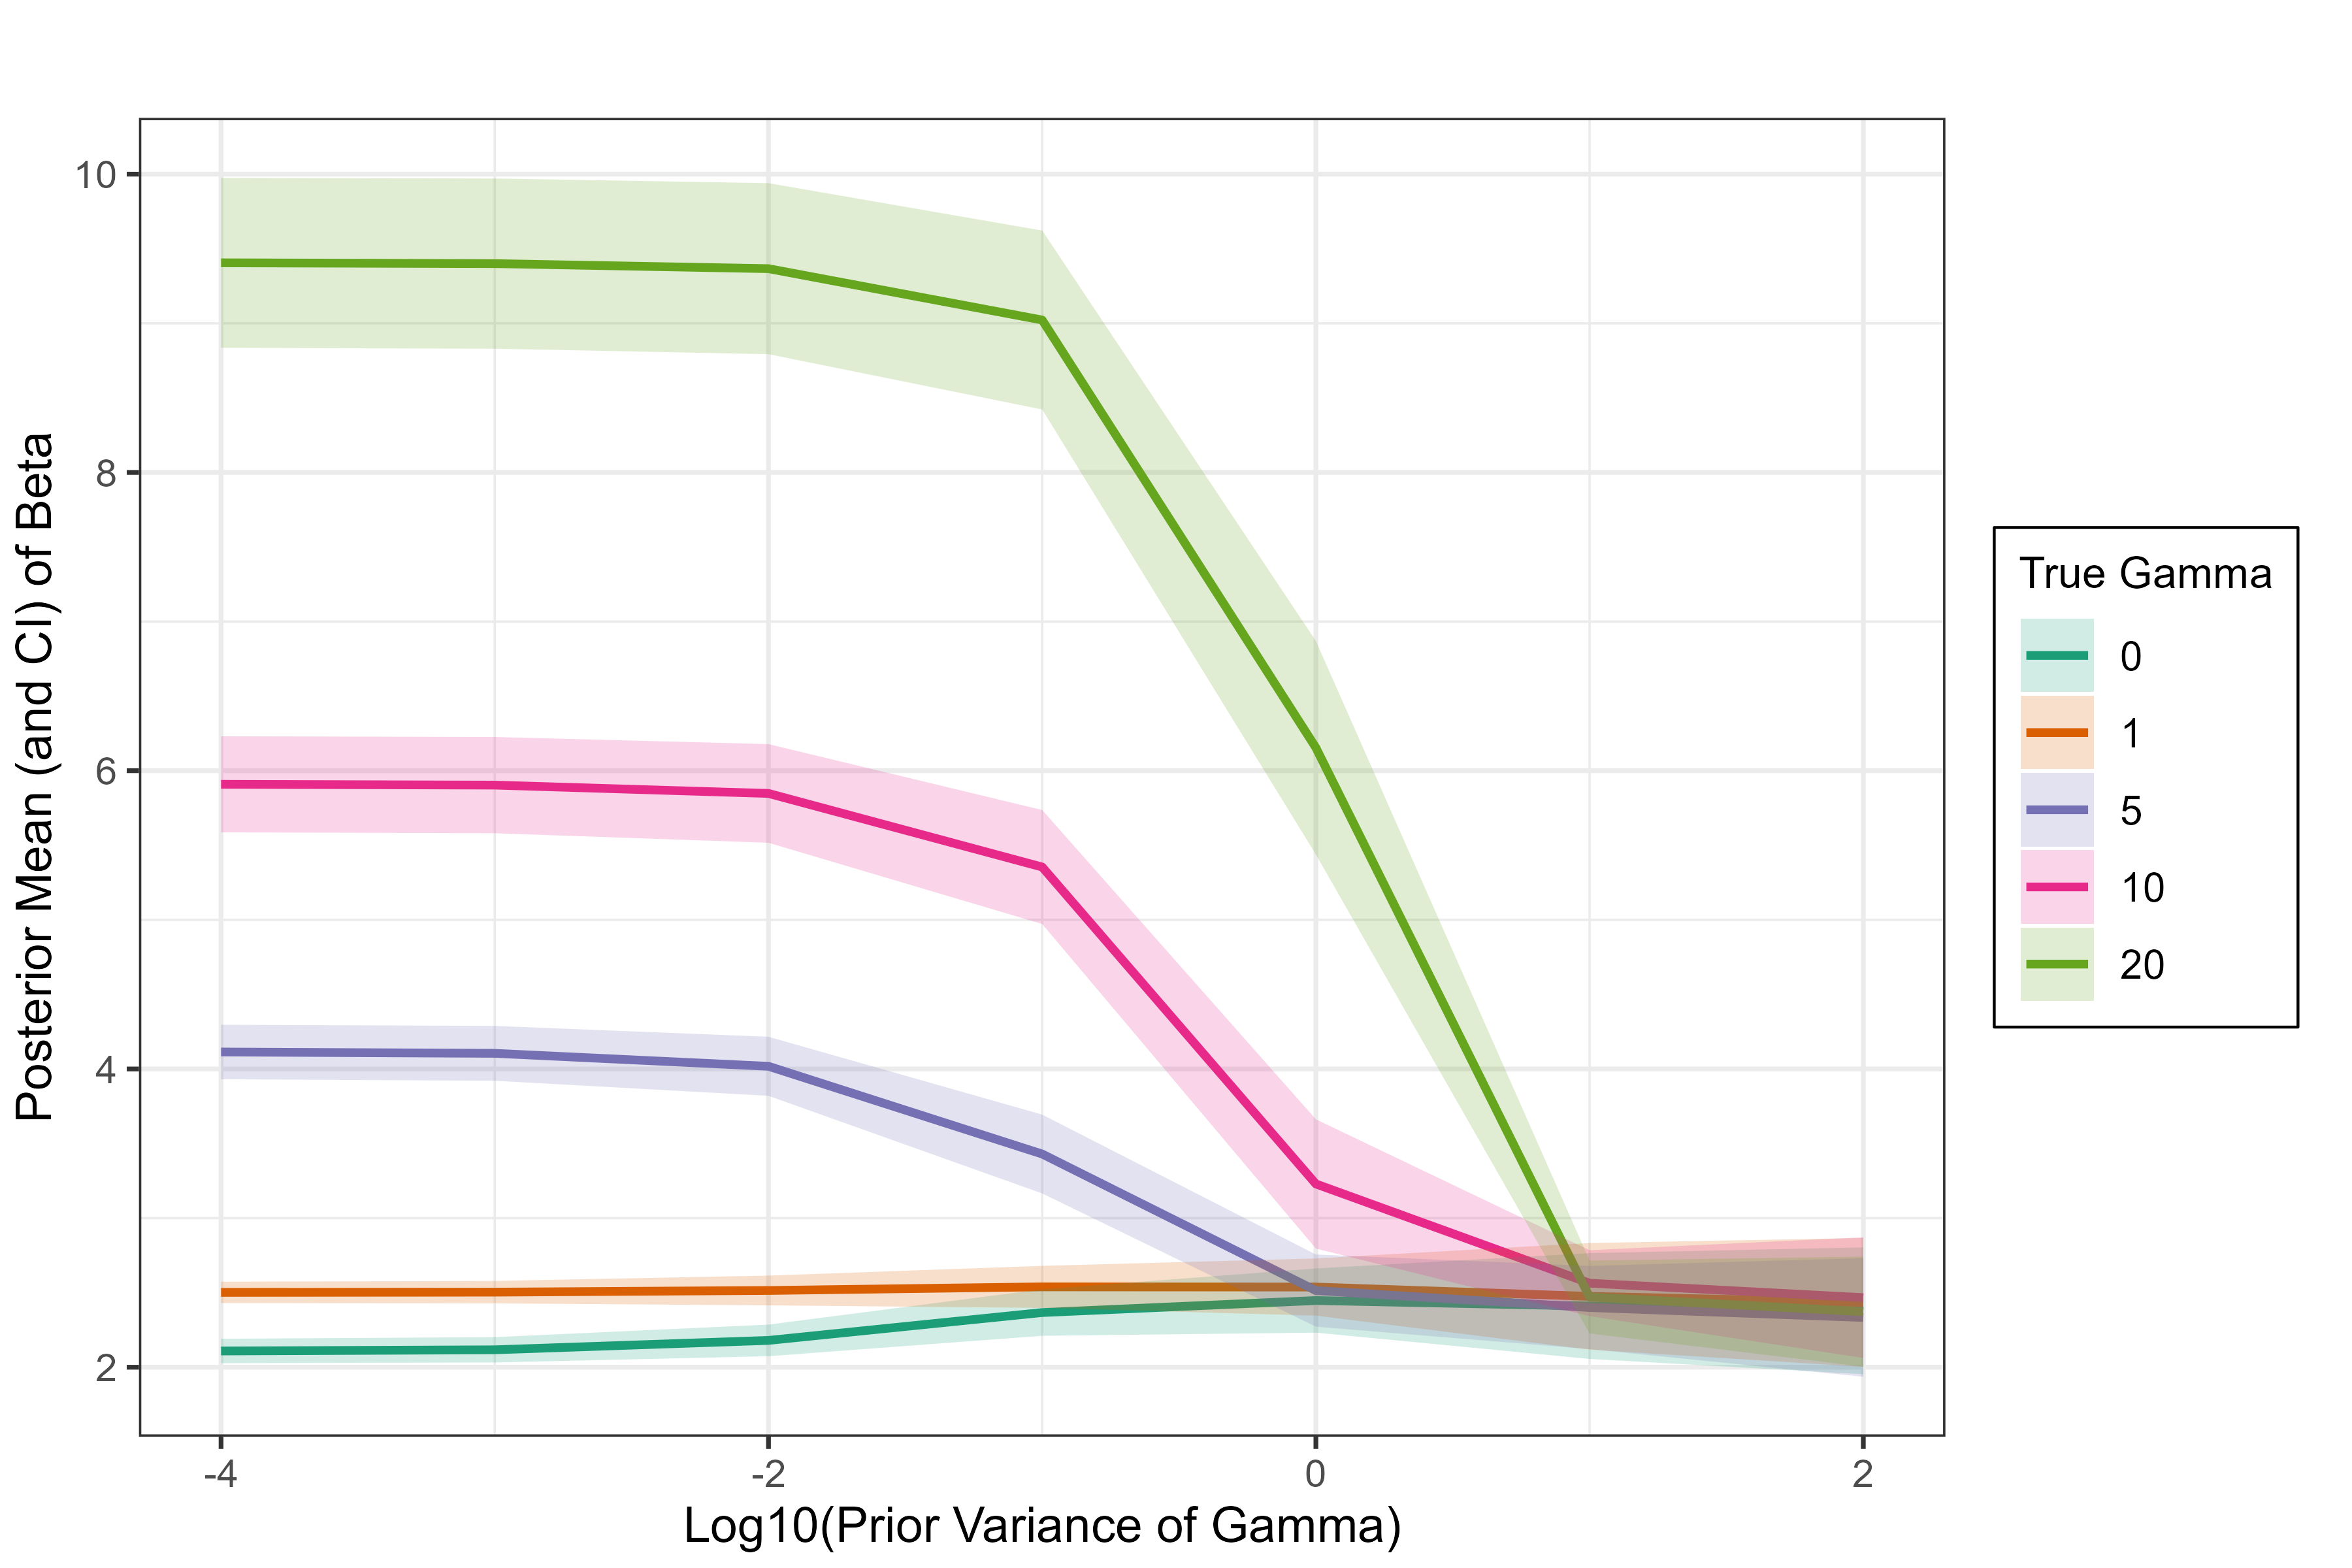
\includegraphics[width=0.9\textwidth]{../figures/simulation/plot_prior_gamma.png}
\caption{Sensitivity Analysis of $\widehat{\beta}$ to Prior Variance of $\gamma$ --- Simulation Study}
\label{fig:sensitivity_analysis_beta}
\end{figure}

As we can see, when the prior variance is very small, we firmly believe that $\gamma$ is equal to 0, and the posterior mean of $\beta$ is close to the true value. If this were to be false, we would be far away from $\beta$ true value, as occurs for different values of $\gamma$. However, as we impose a less informative prior, by increasing the prior variance of $\gamma$, allowing for a non-zero coefficient for the instrument, we see that the posterior mean of $\beta$ converge to a biased estimate which is the same for all true values of $\gamma$. This is because the prior variance is so large that it dominates the likelihood, and the posterior mean of $\beta$ is driven by the prior.